\documentclass[11pt,a4paper,openany]{report}
% ---------------------------------------------------------------------------
% Preâmbulo da apostila do GHOST.
% Fontes da identidade visual em fontes/.
% Compilar com XeLaTeX.
% ---------------------------------------------------------------------------

\usepackage{fontspec}
\usepackage{unicode-math}
\usepackage{polyglossia}
\setdefaultlanguage{portuguese}

\usepackage[a4paper,top=2.7cm,bottom=2.6cm,left=2.9cm,right=2.9cm,
            headsep=1.0cm,footskip=1.3cm]{geometry}
\usepackage{microtype}
\usepackage{xcolor}
\usepackage{tikz}
\usepackage{pgfplots}
\pgfplotsset{compat=1.18}
\usetikzlibrary{calc,positioning,arrows.meta,decorations.pathreplacing,
                shapes.geometric,backgrounds,fit,patterns}
\usepackage{booktabs}
\usepackage{array}
\usepackage{enumitem}
\usepackage{titlesec}
\usepackage{titletoc}
\usepackage{fancyhdr}
\usepackage{tcolorbox}
\tcbuselibrary{skins,breakable}
\usepackage{caption}
\usepackage[hidelinks]{hyperref}

% ------------------------------------------------------------------ paleta
\definecolor{navy}{HTML}{071B2C}
\definecolor{navyfundo}{HTML}{04121E}
\definecolor{cyan}{HTML}{8DD7DC}
\definecolor{gold}{HTML}{E6B75C}
\definecolor{areia}{HTML}{F6F3EC}
\definecolor{anil}{HTML}{A9AEF0}
% derivadas, para tinta sobre papel claro
\definecolor{tinta}{HTML}{10222F}
\definecolor{cyanescuro}{HTML}{1F6B73}
\definecolor{goldescuro}{HTML}{9A6F1E}
\definecolor{anilescuro}{HTML}{4A4FA8}
\definecolor{grafite}{HTML}{5C6B74}
\definecolor{linha}{HTML}{D6DDD8}
\definecolor{papel}{HTML}{FBFAF6}

% ------------------------------------------------------------------ fontes
\newcommand{\FONTES}{fontes/}
\setmainfont{Newsreader-Regular.ttf}[
  Path            = \FONTES,
  ItalicFont      = Newsreader-Italic.ttf,
  BoldFont        = Newsreader-SemiBold.ttf,
  BoldItalicFont  = Newsreader-SemiBoldItalic.ttf,
  Ligatures       = TeX ]
\setsansfont{Manrope-Regular.ttf}[
  Path            = \FONTES,
  ItalicFont      = Manrope-Regular.ttf,
  BoldFont        = Manrope-SemiBold.ttf,
  BoldItalicFont  = Manrope-SemiBold.ttf,
  Ligatures       = TeX ]
\setmonofont{DMMono-Regular.ttf}[
  Path            = \FONTES,
  ItalicFont      = DMMono-Italic.ttf,
  BoldFont        = DMMono-Medium.ttf,
  BoldItalicFont  = DMMono-MediumItalic.ttf,
  Scale           = 0.86 ]
\newfontfamily\displayfont{Newsreader-Display.ttf}[Path=\FONTES, Ligatures=TeX]
\newfontfamily\manropelight{Manrope-Light.ttf}[Path=\FONTES]
\newfontfamily\manropemed{Manrope-Medium.ttf}[Path=\FONTES]

% Newsreader e DM Mono nao trazem gregas: toda letra grega vem da fonte
% matematica, em modo matematico. Nunca escreva "ν" no texto corrido.
\setmathfont{STIXTwoMath-Regular.otf}

% ------------------------------------------------------------------ titulos
\titleformat{\chapter}[display]
  {\sffamily\bfseries\color{tinta}}
  {\manropelight\fontsize{54}{54}\selectfont\color{cyanescuro}\thechapter}
  {6pt}
  {\fontsize{25}{29}\selectfont\raggedright}
  [{\vspace{4pt}\color{gold}\rule{4.2cm}{2pt}}]
\titlespacing*{\chapter}{0pt}{0pt}{34pt}

\titleformat{\section}{\sffamily\bfseries\large\color{tinta}}{\thesection}{0.7em}{}
\titlespacing*{\section}{0pt}{2.6ex plus .6ex}{1.0ex}
\titleformat{\subsection}{\sffamily\bfseries\normalsize\color{cyanescuro}}{\thesubsection}{0.6em}{}
\titlespacing*{\subsection}{0pt}{2.0ex plus .4ex}{0.6ex}

\setcounter{secnumdepth}{2}
\setcounter{tocdepth}{1}

% ------------------------------------------------------------------ corpo
\setlength{\parskip}{0.55ex}
\setlength{\parindent}{1.1em}
\renewcommand{\arraystretch}{1.24}
\setlist[itemize]{leftmargin=1.3em, itemsep=0.3ex, topsep=0.6ex, label=\color{cyanescuro}\textbullet}
\setlist[enumerate]{leftmargin=1.5em, itemsep=0.4ex, topsep=0.6ex}
\setlist[description]{leftmargin=0pt, font=\sffamily\bfseries\color{tinta}}

% Figuras devem ficar perto do texto que as explica: numa apostila, uma
% figura que migra tres paginas deixa de ser a figura daquele paragrafo.
\renewcommand{\topfraction}{0.92}
\renewcommand{\bottomfraction}{0.85}
\renewcommand{\textfraction}{0.06}
\renewcommand{\floatpagefraction}{0.80}
\setcounter{topnumber}{3}
\setcounter{bottomnumber}{2}
\setcounter{totalnumber}{4}

\captionsetup{font={sf,small}, labelfont={bf,color=cyanescuro}, width=0.92\linewidth}

\pagestyle{fancy}
\fancyhf{}
\renewcommand{\headrulewidth}{0pt}
\fancyhead[L]{\sffamily\scriptsize\color{grafite}\textsc{ghost}}
\fancyhead[R]{\sffamily\scriptsize\color{grafite}\nouppercase{\leftmark}}
\fancyfoot[C]{\sffamily\small\color{grafite}\thepage}
\fancypagestyle{plain}{\fancyhf{}\renewcommand{\headrulewidth}{0pt}%
  \fancyfoot[C]{\sffamily\small\color{grafite}\thepage}}

\hypersetup{colorlinks=true, linkcolor=cyanescuro, urlcolor=cyanescuro,
  pdftitle={GHOST -- uma apostila para comecar},
  pdfsubject={Oscilacao de neutrinos: sabor, materia e decoerencia},
  pdfauthor={Rafael C. R. de Lima}}

% ------------------------------------------------------------------ caixas
\newtcolorbox{nota}[1][]{
  enhanced, colback=papel, colframe=linha, boxrule=0.5pt,
  arc=1.5pt, left=9pt, right=9pt, top=7pt, bottom=7pt,
  borderline west={2.2pt}{-2.2pt}{cyanescuro}, #1}

\newtcolorbox{alerta}[1][]{
  enhanced, colback=papel, colframe=linha, boxrule=0.5pt,
  arc=1.5pt, left=9pt, right=9pt, top=7pt, bottom=7pt,
  borderline west={2.2pt}{-2.2pt}{goldescuro}, #1}

\newtcolorbox{conceito}[1][]{
  enhanced, colback=navy, colframe=navy, boxrule=0pt,
  arc=2pt, left=11pt, right=11pt, top=9pt, bottom=9pt,
  coltext=areia, fontupper=\linespread{1.15}\selectfont, #1}

% rótulo de caixa
\newcommand{\rotulo}[1]{{\sffamily\bfseries\footnotesize\color{cyanescuro}\MakeUppercase{#1}}\par\vspace{2pt}}
\newcommand{\rotuloa}[1]{{\sffamily\bfseries\footnotesize\color{goldescuro}\MakeUppercase{#1}}\par\vspace{2pt}}
\newcommand{\rotuloc}[1]{{\sffamily\bfseries\footnotesize\color{cyan}\MakeUppercase{#1}}\par\vspace{2pt}}

% ------------------------------------------------------------------ atalhos
\newcommand{\nue}{\nu_e}
\newcommand{\numu}{\nu_\mu}
\newcommand{\nutau}{\nu_\tau}
\newcommand{\Losc}{L_{\text{osc}}}
\newcommand{\PH}{P_H}
\newcommand{\dm}[1]{\Delta m^2_{#1}}
\newcommand{\cmd}[1]{{\ttfamily #1}}
\newcommand{\ket}[1]{\left|#1\right\rangle}
\newcommand{\bra}[1]{\left\langle#1\right|}
\newcommand{\braket}[2]{\left\langle#1\middle|#2\right\rangle}

% Espacejamento de letras: no XeLaTeX vem do fontspec, nao do microtype.
\newfontfamily\espacejada{Manrope-SemiBold.ttf}[Path=\FONTES, LetterSpace=22.0]

\begin{document}

% ---------------------------------------------------------------------------
% Capa. Sangria total em navy, com o cruzamento evitado desenhado ao fundo:
% as duas curvas que quase se tocam SAO o assunto do documento.
% ---------------------------------------------------------------------------
\begin{titlepage}
\thispagestyle{empty}
\begin{tikzpicture}[remember picture, overlay]

  % fundo
  \fill[navyfundo] (current page.south west) rectangle (current page.north east);

  % campo de raios tenue, saindo do canto superior direito: a supernova
  \begin{scope}
    \clip (current page.south west) rectangle (current page.north east);
    \foreach \a in {188,194,...,268}{
      \draw[cyan, opacity=0.07, line width=0.5pt]
        ($(current page.north east)+(0.6,0.6)$) -- ++(\a:32cm);
    }
    \foreach \r in {5,9,...,29}{
      \draw[cyan, opacity=0.05, line width=0.4pt]
        ($(current page.north east)+(0.6,0.6)$) circle (\r cm);
    }
  \end{scope}

  % ---- o cruzamento evitado, elemento central -----------------------------
  % Dois autovalores em funcao da densidade. Longe da ressonancia eles seguem
  % as assintotas; perto dela se repelem. E a figura do capitulo 3.
  \begin{scope}[shift={($(current page.center)+(0,-3.95)$)}, x=1cm, y=1cm]
    % Assintotas: os estados de SABOR, que se cruzariam sem mistura.
    % Para y = 0.289x +- sqrt(0.0835x^2 + 0.30), as assintotas sao exatamente
    % y = 0 e y = 0.578x. Desenhar outra coisa seria desenhar outra fisica.
    \draw[areia, opacity=0.18, line width=0.6pt, dash pattern=on 2pt off 2.6pt]
      (-6.4,0) -- (6.4,0);
    \draw[areia, opacity=0.18, line width=0.6pt, dash pattern=on 2pt off 2.6pt]
      (-6.4,-3.70) -- (6.4,3.70);
    % ramos de fato (autovalores em materia)
    \draw[cyan, line width=1.5pt]
      plot[domain=-6.4:6.4, samples=220] (\x, {0.289*\x + sqrt(0.0835*\x*\x + 0.30)});
    \draw[gold, line width=1.5pt]
      plot[domain=-6.4:6.4, samples=220] (\x, {0.289*\x - sqrt(0.0835*\x*\x + 0.30)});
    % a separacao minima
    \draw[areia, opacity=0.5, line width=0.5pt] (0,0.548) -- (0,-0.548);
    \fill[areia, opacity=0.85] (0,0.548) circle (1.5pt);
    \fill[areia, opacity=0.85] (0,-0.548) circle (1.5pt);
    \node[areia, opacity=0.62, font=\sffamily\tiny, right=5pt] at (0.1,0)
      {ressonância};
  \end{scope}

  % ---- texto --------------------------------------------------------------
  \node[anchor=north west, text=cyan, font=\espacejada\footnotesize]
    at ($(current page.north west)+(2.9,-2.6)$)
    {APOSTILA PARA COMEÇAR};

  \node[anchor=north west, inner sep=0pt]
    at ($(current page.north west)+(2.88,-3.35)$)
    {\parbox{15cm}{\raggedright
       {\displayfont\fontsize{74}{74}\selectfont\color{areia} GHOST}\\[10pt]
       {\displayfont\fontsize{21}{27}\selectfont\color{cyan}
        Oscilação de neutrinos:\\ sabor, matéria e decoerência}}};

  \node[anchor=north west, inner sep=0pt]
    at ($(current page.north west)+(2.95,-8.5)$)
    {\tikz\draw[gold, line width=2.2pt] (0,0) -- (3.6,0);};

  \node[anchor=north west, inner sep=0pt]
    at ($(current page.north west)+(2.88,-9.3)$)
    {\parbox{12.2cm}{\raggedright\sffamily\color{areia}\fontsize{10.2}{15.6}\selectfont
       Um neutrino de $n$ sabores é um sistema de $n$ níveis com hamiltoniano
       hermitiano. O núcleo do GHOST propaga
       $\ket{\psi(t)}=e^{-iHt}\ket{\psi(0)}$ por expansão de Chebyshev, para
       $H$ qualquer --- esparsa e hermitiana. Oscilação de sabor é um caso
       particular. Esta apostila leva esse caso a sério, do início.}};

  % rodape
  \node[anchor=south west, inner sep=0pt]
    at ($(current page.south west)+(2.88,2.05)$)
    {\parbox{13cm}{\raggedright\sffamily\color{areia}\fontsize{9.4}{14}\selectfont
       \textbf{Rafael C. R. de Lima}\\
       {\color{cyan}Universidade do Estado de Santa Catarina\,\textperiodcentered\,ICRANet}}};

  \node[anchor=south east, inner sep=0pt]
    at ($(current page.south east)+(-2.88,2.05)$)
    {\sffamily\color{grafite}\footnotesize \today};

  \draw[cyan, opacity=0.30, line width=0.6pt]
    ($(current page.south west)+(2.88,3.0)$) -- ($(current page.south east)+(-2.88,3.0)$);

\end{tikzpicture}
\end{titlepage}


% ---- sumario -------------------------------------------------------------
\thispagestyle{empty}
\vspace*{1.2cm}
{\sffamily\bfseries\LARGE\color{tinta}Sumário}\par
\vspace{2pt}{\color{gold}\rule{3.2cm}{2pt}}\par
\vspace{1.0cm}
{\titlecontents{chapter}[0em]
  {\vspace{1.1ex}\sffamily\bfseries\color{tinta}}
  {\color{cyanescuro}\thecontentslabel\hspace{0.8em}}{}
  {\;\titlerule*[0.6pc]{.}\;\color{grafite}\thecontentspage}
 \titlecontents{section}[1.6em]
  {\vspace{0.15ex}\small\color{grafite}}
  {\thecontentslabel\hspace{0.6em}}{}
  {\;\titlerule*[0.6pc]{.}\;\thecontentspage}
 \makeatletter\@starttoc{toc}\makeatother}
\clearpage

\chapter{De onde veio a pergunta}
\markboth{História}{História}

Este capítulo não é decoração. Quase todo erro que você vai cometer nos
primeiros meses já foi cometido por alguém entre 1930 e 2005, e a forma do erro
está registrada. Vale saber onde.

\section{Uma partícula inventada para salvar uma conta}

Em dezembro de 1930 Wolfgang Pauli escreveu a uma reunião em Tübingen propondo
uma partícula neutra, leve e quase inerte, emitida junto com o elétron no
decaimento beta. O espectro do elétron era contínuo, e num decaimento de dois
corpos ele deveria ser uma linha. Ou a energia não se conservava --- que era a
alternativa que Bohr considerava seriamente --- ou faltava alguém levando o
resto.

Pauli chamou sua proposta de \emph{remédio desesperado} e escreveu que tinha
feito algo que um teórico não deveria: postular uma partícula que, pelos seus
próprios cálculos, ninguém conseguiria detectar. Ele estava errado, mas por
pouco: foram vinte e seis anos.

\begin{nota}
\rotulo{o que fica disso}
A seção de choque do neutrino é pequena porque a interação é fraca, e é essa
mesma pequenez que o torna útil. Um fóton emitido no centro de uma estrela leva
milhares de anos para sair. Um neutrino sai em segundos. \textbf{É a única
sonda que atravessa.}
\end{nota}

Em 1956 Clyde Cowan e Frederick Reines puseram detectores de cintilador líquido
junto ao reator de Savannah River e mediram o decaimento beta inverso,
$\bar\nue + p \to n + e^+$. Mandaram um telegrama a Pauli. A partícula existia.

\section{O problema solar, e ele durou trinta anos}

Nos anos 1960 Raymond Davis instalou um tanque de 615 toneladas de
percloroetileno na mina de Homestake, em Dakota do Sul --- a mesma mina onde
hoje se constrói o detector distante do DUNE --- para contar neutrinos do Sol
pela reação $\nue + {}^{37}\text{Cl} \to {}^{37}\text{Ar} + e^-$. John Bahcall
calculou quantos deveriam chegar.

Davis media cerca de um terço da previsão. E mediu isso, com a mesma resposta,
por três décadas.

A comunidade passou anos dividida entre duas explicações naturais e uma
estranha. A natural era que o modelo solar estivesse errado --- a taxa depende
muito fortemente da temperatura central. A outra natural era que o experimento
tivesse um problema. A estranha, levantada por Bruno Pontecorvo já em 1957 e
elaborada por Maki, Nakagawa e Sakata em 1962, era que o neutrino \emph{mudasse
de identidade no caminho}.

\begin{alerta}
\rotuloa{o padrão que se repete}
A hipótese estranha venceu, mas só depois que a heliossismologia fechou a porta
do modelo solar e que um segundo tipo de experimento mediu a coisa de outro
jeito. \textbf{Uma anomalia num único canal não resolve nada.} É o mesmo
argumento que aparece no capítulo~\ref{cap:fronteira} quando se discute o que o
GHOST pode e o que não pode afirmar sozinho.
\end{alerta}

\section{Dois anúncios que fecharam a questão}

\begin{description}
\item[1987.] Em 23 de fevereiro, Kamiokande-II, IMB e Baksan registraram, em
  cerca de treze segundos, vinte e quatro eventos de neutrino. Horas depois a
  supernova SN~1987A apareceu na Grande Nuvem de Magalhães. É o único evento de
  neutrinos de supernova já detectado, e praticamente tudo que sabemos
  \emph{observacionalmente} sobre o colapso de um núcleo estelar vem daqueles
  vinte e quatro eventos.

\item[1998.] O Super-Kamiokande mostrou que neutrinos atmosféricos produzidos do
  outro lado da Terra chegavam em menor número que os produzidos logo acima ---
  uma dependência com a distância percorrida, que é a assinatura de oscilação e
  não de um erro de fluxo.

\item[2002.] O SNO mediu o fluxo solar de duas maneiras: pelo canal de corrente
  carregada, sensível só a $\nue$, e pelo canal de corrente neutra, sensível aos
  três sabores igualmente. O fluxo total batia com Bahcall. O de $\nue$ era um
  terço. Os neutrinos não sumiam; viravam outra coisa.
\end{description}

Davis e Masatoshi Koshiba dividiram o Nobel de 2002; Takaaki Kajita e Arthur
McDonald, o de 2015. Como oscilar exige massa, e o Modelo Padrão foi construído
com neutrinos sem massa, esta é até hoje a única evidência de laboratório de
física além dele.

\section{A matéria muda o problema}

Em 1978 Lincoln Wolfenstein notou que um $\nue$ atravessando matéria comum
espalha para a frente coerentemente nos elétrons do meio por corrente carregada
--- e $\numu$ e $\nutau$ não, porque não há múons nem taus por perto para
trocar. A matéria adiciona um potencial \emph{a uma única entrada} do
hamiltoniano.

Em 1985 Stanislav Mikheyev e Alexei Smirnov viram a consequência: se a densidade
varia ao longo do caminho, existe um ponto onde esse potencial cancela a
separação de vácuo, e ali os dois níveis chegam à sua aproximação máxima. A
conversão pode ser quase total mesmo com ângulo de mistura pequeno. É o efeito
MSW, e é ele que explica o déficit solar --- e o que este código calcula.

\begin{conceito}
\rotuloc{o fio da meada}
Pauli inventa a partícula para salvar a conservação de energia. Reines e Cowan a
encontram. Davis mede um terço do previsto. Pontecorvo sugere que ela mude de
identidade. Wolfenstein mostra que a matéria quebra a simetria entre os sabores.
Mikheyev e Smirnov mostram que uma densidade \emph{variável} produz conversão
ressonante. SN~1987A entrega os únicos dados. SNO fecha a questão.

\medskip
O GHOST entra no ponto em que a densidade deixa de ser suave: uma supernova real
tem um choque, e o choque atravessa a ressonância.
\end{conceito}

\section{A linha do tempo}

\begin{center}
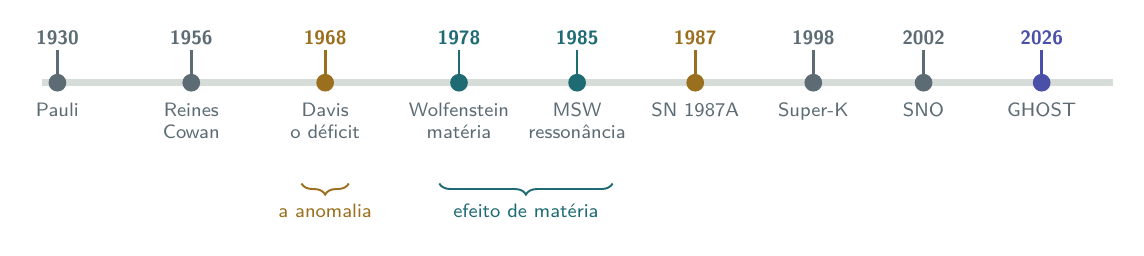
\begin{tikzpicture}[x=1cm, y=1cm]
  \def\Y{0}
  \draw[linha, line width=2.4pt] (0,\Y) -- (13.6,\Y);

  % marcos: posicao / ano / rotulo curto / cor
  \foreach \x/\ano/\txt/\c in {%
      0.2/1930/{Pauli}/grafite,
      1.9/1956/{Reines\\Cowan}/grafite,
      3.6/1968/{Davis\\o déficit}/goldescuro,
      5.3/1978/{Wolfenstein\\matéria}/cyanescuro,
      6.8/1985/{MSW\\ressonância}/cyanescuro,
      8.3/1987/{SN 1987A}/goldescuro,
      9.8/1998/{Super-K}/grafite,
      11.2/2002/{SNO}/grafite,
      12.7/2026/{GHOST}/anilescuro}{
    \fill[\c] (\x,\Y) circle (3.2pt);
    \draw[\c, line width=1pt] (\x,\Y) -- (\x,\Y+0.42);
    \node[anchor=south, font=\sffamily\bfseries\scriptsize, text=\c,
          align=center, inner sep=1pt] at (\x,\Y+0.44) {\ano};
    \node[anchor=north, font=\sffamily\scriptsize, text=grafite,
          align=center, inner sep=3pt] at (\x,\Y-0.14) {\txt};
  }

  % as duas faixas conceituais
  \draw[decorate, decoration={brace, amplitude=4pt, mirror}, cyanescuro,
        line width=0.7pt] (5.05,\Y-1.28) -- (7.25,\Y-1.28);
  \node[anchor=north, font=\sffamily\scriptsize, text=cyanescuro]
    at (6.15,\Y-1.42) {efeito de matéria};

  \draw[decorate, decoration={brace, amplitude=4pt, mirror}, goldescuro,
        line width=0.7pt] (3.3,\Y-1.28) -- (3.9,\Y-1.28);
  \node[anchor=north, font=\sffamily\scriptsize, text=goldescuro]
    at (3.6,\Y-1.42) {a anomalia};
\end{tikzpicture}
\par\vspace{6pt}
\captionof{figure}{Noventa e seis anos. Em dourado, as medidas que não fechavam; em
ciano, a teoria que explicou por quê. O GHOST fica no fim porque a pergunta
dele --- o que acontece quando a densidade \emph{não} é suave --- só faz sentido
depois de todo o resto.}
\end{center}

\chapter{A teoria, do começo}
\label{cap:teoria}
\markboth{Teoria}{Teoria}

Tudo que segue cabe em uma frase: \textbf{o neutrino tem dois conjuntos de
estados, e eles discordam.}

\section{Sabor e massa}

Os estados de \emph{sabor} $\ket{\nue}$, $\ket{\numu}$, $\ket{\nutau}$ são
definidos pelo lépton carregado com que a partícula é produzida ou detectada.
É o que um detector mede: o argônio enxerga $\nue$ porque a reação
$\nue + {}^{40}\text{Ar} \to e^- + {}^{40}\text{K}^*$ produz um elétron.

Os estados de \emph{massa} $\ket{\nu_1}$, $\ket{\nu_2}$, $\ket{\nu_3}$ são os
que têm energia definida, e portanto os que propagam com fase simples.

Os dois conjuntos não coincidem. Uma matriz unitária $U$ --- a matriz PMNS, de
Pontecorvo, Maki, Nakagawa e Sakata --- liga um ao outro:
\begin{equation}
  \ket{\nu_\alpha} = \sum_{i} U_{\alpha i}^{*}\,\ket{\nu_i},
  \qquad \alpha \in \{e,\mu,\tau\},\quad i \in \{1,2,3\}.
\end{equation}

\begin{figure}[!htb]
\centering
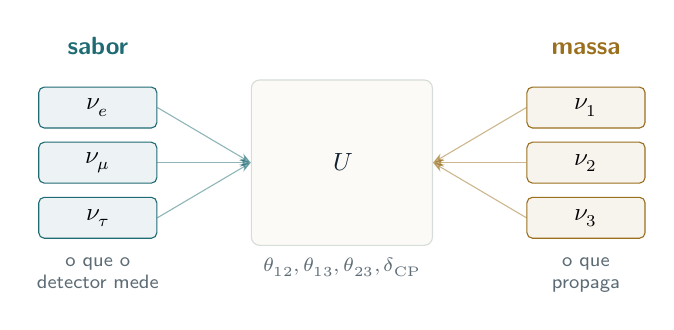
\begin{tikzpicture}[x=1cm, y=1cm, font=\sffamily\small]
  % sabor
  \node[anchor=south, font=\sffamily\bfseries\small, text=cyanescuro] at (0,2.55) {sabor};
  \foreach \i/\y/\n in {a/2.0/{$\nu_e$}, b/1.3/{$\nu_\mu$}, c/0.6/{$\nu_\tau$}}{
    \node[draw=cyanescuro, fill=cyanescuro!8, rounded corners=2pt,
          minimum width=1.5cm, minimum height=0.52cm, font=\small] (f\i) at (0,\y) {\n};}
  \node[anchor=north, text=grafite, font=\sffamily\scriptsize, align=center]
    at (0,0.22) {o que o\\detector mede};

  % massa
  \node[anchor=south, font=\sffamily\bfseries\small, text=goldescuro] at (6.2,2.55) {massa};
  \foreach \i/\y/\n in {a/2.0/{$\nu_1$}, b/1.3/{$\nu_2$}, c/0.6/{$\nu_3$}}{
    \node[draw=goldescuro, fill=goldescuro!8, rounded corners=2pt,
          minimum width=1.5cm, minimum height=0.52cm, font=\small] (m\i) at (6.2,\y) {\n};}
  \node[anchor=north, text=grafite, font=\sffamily\scriptsize, align=center]
    at (6.2,0.22) {o que\\propaga};

  % a matriz entre os dois
  \node[draw=linha, fill=papel, rounded corners=3pt, minimum width=2.3cm,
        minimum height=2.1cm, font=\sffamily\bfseries\small, text=tinta] (U) at (3.1,1.3) {$U$};
  \node[anchor=north, text=grafite, font=\sffamily\scriptsize, align=center]
    at (3.1,0.22) {$\theta_{12},\theta_{13},\theta_{23},\delta_{\rm CP}$};

  \foreach \i in {a,b,c}{
    \draw[cyanescuro, opacity=0.5, -{Stealth[length=4pt]}] (f\i.east) -- (U.west);
    \draw[goldescuro, opacity=0.5, {Stealth[length=4pt]}-] (U.east) -- (m\i.west);}
\end{tikzpicture}
\caption{Os dois conjuntos de estados e a rotação entre eles. Três ângulos e
uma fase descrevem $U$ inteira. Toda a fenomenologia de oscilação é a
consequência de produzir na base da esquerda, propagar na base da direita, e
perguntar de novo na da esquerda.}
\end{figure}

\section{Oscilação no vácuo}

Massas diferentes acumulam fase a taxas diferentes. Um estado criado como
$\nue$ puro é, depois de percorrer $L$, uma superposição distinta; perguntar de
novo pelo sabor pode dar outra resposta. No caso de dois sabores,
\begin{equation}
  P(\nue \to \nue) = 1 - \sin^2 2\theta \,
    \sin^2\!\left(\frac{\pi L}{\Losc}\right),
  \qquad
  \Losc = \frac{4\pi E}{\Delta m^2}.
\end{equation}

Em unidades práticas,
\begin{equation}
  \Losc[\text{m}] = 2{,}48\;\frac{E[\text{MeV}]}{\Delta m^2[\text{eV}^2]},
\end{equation}
onde o $2{,}48$ é para onde foi o $\hbar c$. Guarde esse número: ele aparece em
toda estimativa de ordem de grandeza daqui para a frente. Para
$E = 20\ \text{MeV}$ e $\dm{31} = 2{,}51\times10^{-3}\ \text{eV}^2$, dá
$\Losc \simeq 19{,}8$~km.

\begin{figure}[!htb]
\centering
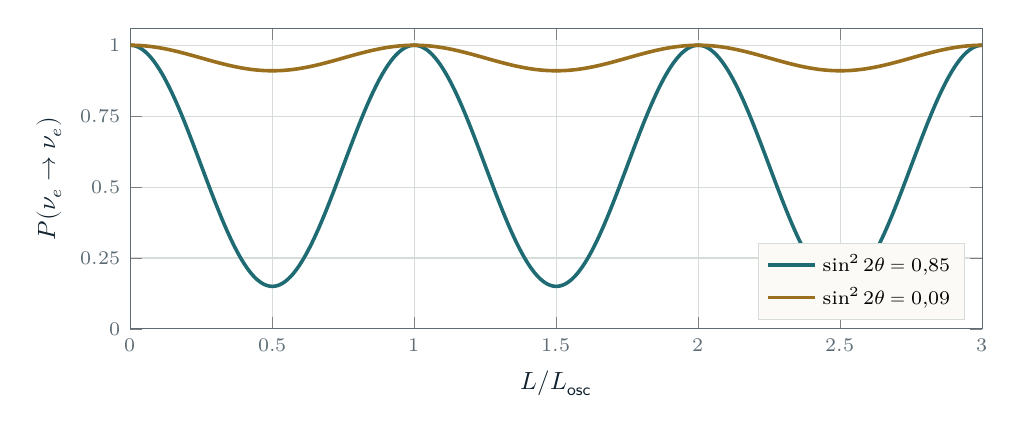
\begin{tikzpicture}
\begin{axis}[
  width=12.4cm, height=5.4cm,
  xlabel={$L/\Losc$}, ylabel={$P(\nue\to\nue)$},
  xmin=0, xmax=3, ymin=0, ymax=1.06,
  xtick={0,0.5,1,1.5,2,2.5,3}, ytick={0,0.25,0.5,0.75,1},
  grid=major, grid style={linha, line width=0.4pt},
  tick label style={font=\sffamily\scriptsize, color=grafite},
  label style={font=\sffamily\small, color=tinta},
  axis line style={grafite}, legend style={font=\sffamily\scriptsize,
    draw=linha, fill=papel, at={(0.98,0.03)}, anchor=south east},
]
\addplot[cyanescuro, line width=1.3pt, domain=0:3, samples=400]
  {1 - 0.85*sin(deg(pi*x))^2};
\addlegendentry{$\sin^2 2\theta = 0{,}85$}
\addplot[goldescuro, line width=1.3pt, domain=0:3, samples=400]
  {1 - 0.09*sin(deg(pi*x))^2};
\addlegendentry{$\sin^2 2\theta = 0{,}09$}
\end{axis}
\end{tikzpicture}
\caption{Oscilação no vácuo. O ângulo de mistura fixa a \emph{profundidade} do
vale; a razão $L/E$ fixa \emph{onde} ele cai. Com ângulo pequeno a conversão no
vácuo é fraca --- e é exatamente essa a situação que o efeito de matéria vira
do avesso.}
\end{figure}

\section{Dentro da matéria, o problema não é o mesmo}
\label{sec:materia}

Acrescente o potencial de Wolfenstein à entrada $\nue$ do hamiltoniano:
\begin{equation}
  H(r) = \underbrace{\frac{1}{2E}\,U
      \operatorname{diag}\!\left(0,\ \dm{21},\ \dm{31}\right) U^{\dagger}}_{\text{vácuo: fixo}}
    + \underbrace{\operatorname{diag}\!\left(\sqrt{2}\,G_F\,\frac{Y_e\,\rho(r)}{m_N},
      \ 0,\ 0\right)}_{\text{matéria: depende de onde o neutrino está}}.
\label{eq:hamiltoniano}
\end{equation}

É esta a matriz que o GHOST integra, e ela merece ser desmontada peça por peça
--- é a equação de que tudo o mais neste documento é consequência.

\subsection{De onde vem o primeiro termo}

Um neutrino relativístico de momento $p$ e massa $m_i$ tem energia
\begin{equation}
  E_i = \sqrt{p^2 + m_i^2} \;\simeq\; p + \frac{m_i^2}{2p}
   \;\simeq\; E + \frac{m_i^2}{2E},
\end{equation}
porque $m_i \ll p$ --- para $m \lesssim 0{,}1$~eV e $E \sim 10$~MeV a razão é
$10^{-8}$. Na base de massa a evolução é uma fase por estado,
$\ket{\nu_i(t)} = e^{-iE_i t}\ket{\nu_i(0)}$, logo o gerador é
$\operatorname{diag}(m_1^2, m_2^2, m_3^2)/2E$, a menos do termo comum $E$.

Esse termo comum é proporcional à identidade. \textbf{Uma fase global não é
observável}, então ele sai --- e, pela mesma razão, pode-se subtrair
$m_1^2/2E$ de todos, o que deixa
$\operatorname{diag}(0,\ \dm{21},\ \dm{31})/2E$. É por isso que só aparecem
\emph{diferenças} de massa ao quadrado: são as únicas coisas que a oscilação
consegue enxergar.

Falta ir para a base em que o detector pergunta. A rotação
$H_{\alpha\beta} = \sum_i U_{\alpha i}\,\lambda_i\,U^{*}_{\beta i}$, com
$\lambda = (0, \dm{21}, \dm{31})/2E$, é literalmente o laço triplo que o código
executa.

\subsection{De onde vem o segundo}

Atravessando matéria, o neutrino espalha para a frente \emph{coerentemente} ---
sem perder energia e sem mudar de direção, apenas acumulando fase, como luz
atravessando vidro. Isso é um índice de refração, e um índice de refração é um
potencial.

Todo sabor espalha por corrente neutra, e igualmente. Um termo proporcional à
identidade, de novo, não faz nada. Mas só o $\nue$ espalha por \emph{corrente
carregada}, trocando um $W$ com os elétrons do meio --- porque não há múons nem
taus por perto para o $\numu$ e o $\nutau$ trocarem. Sobra
\begin{equation}
  V_{\rm CC} = \sqrt{2}\,G_F\,n_e,
  \qquad n_e = \frac{Y_e\,\rho}{m_N},
\end{equation}
em uma única entrada. $Y_e$ é a fração de elétrons por bárion, e $m_N$ a massa
do núcleon.

\begin{nota}
\rotulo{a constante, em número}
Juntando $G_F$, $(\hbar c)^3$ e $m_N$, o potencial em eV por unidade de
$Y_e\,\rho$ em g\,cm$^{-3}$ vale
\[
  \frac{\sqrt{2}\,G_F (\hbar c)^3}{m_N}
  = 7{,}566899624856641\times10^{-14}\ \text{eV}\ \frac{\text{cm}^3}{\text{g}}.
\]
É a \cmd{DAE\_NU\_V\_POR\_RHO} do \cmd{dae\_neutrino.h}, e ela é
\emph{derivada} das constantes, não tabelada --- o comentário no código diz
isso explicitamente. Note que a massa usada é a do \textbf{nêutron}, não a
unidade de massa atômica: a escolha muda o valor em $0{,}87\%$, e trocá-la
``corrigindo'' para $m_u$ desloca a ressonância.
\end{nota}

Para antineutrinos o sinal de $V$ inverte, o que é a razão física de a
ressonância morar no setor de neutrinos com ordenamento normal e no de
antineutrinos com invertido.

\subsection{A ressonância, com o número}

Um neutrino que sai do núcleo de uma estrela viaja para fora, atravessando
densidade decrescente. Na densidade em que o potencial de matéria cancela a
separação de vácuo --- isto é, em
$V = (\dm{31}/2E)\cos 2\theta_{13}$ --- os dois níveis atingem sua aproximação
máxima.

Vale a pena fazer essa conta uma vez na vida. Com $\dm{31} = 2{,}51\times10^{-3}$~eV$^2$,
$E = 20$~MeV e $\theta_{13} = 8{,}6^\circ$:
\begin{align}
  \frac{\dm{31}}{2E} &= \frac{2{,}51\times10^{-3}}{2\times2\times10^{7}}
     = 6{,}275\times10^{-11}\ \text{eV},\\[2pt]
  V_{\rm res} &= 6{,}275\times10^{-11}\times\cos(17{,}2^\circ)
     = 5{,}994\times10^{-11}\ \text{eV},\\[2pt]
  (Y_e\rho)_{\rm res} &= \frac{5{,}994\times10^{-11}}{7{,}5669\times10^{-14}}
     = \mathbf{792}\ \text{g\,cm}^{-3}.
\end{align}

Que é a equação~\eqref{eq:resonancia}, agora com procedência:
\begin{equation}
  Y_e\,\rho_{\rm res} \simeq 792\ \text{g\,cm}^{-3}\,
     \left(\frac{20\ \text{MeV}}{E}\right).
\label{eq:resonancia}
\end{equation}
A dependência em $1/E$ é o que faz a assinatura do choque \emph{migrar através
da energia} conforme a frente se move --- o mapa em $(t,E)$ do
capítulo~\ref{cap:exemplos}.

\subsection{O ângulo de mistura efetivo}

A forma mais limpa de ver o que a matéria faz é diagonalizar
$H$ em densidade constante. Com dois sabores, o ângulo em matéria obedece
\begin{equation}
  \sin^2 2\theta_m = \frac{\sin^2 2\theta}
    {\left(\cos 2\theta - x\right)^2 + \sin^2 2\theta},
  \qquad x \equiv \frac{2E\,V}{\Delta m^2}.
\label{eq:angulo-efetivo}
\end{equation}

\begin{figure}[!htb]
\centering
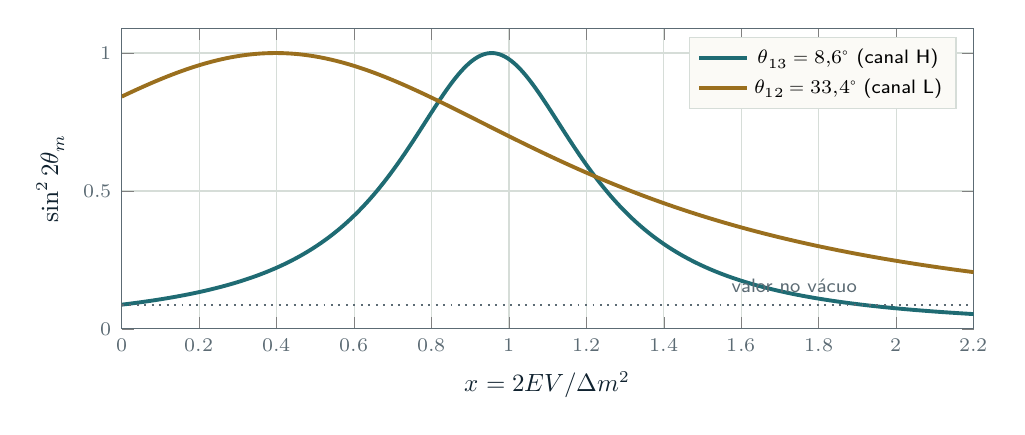
\begin{tikzpicture}
\begin{axis}[
  width=12.4cm, height=5.4cm,
  xlabel={$x = 2EV/\Delta m^2$}, ylabel={$\sin^2 2\theta_m$},
  xmin=0, xmax=2.2, ymin=0, ymax=1.09,
  grid=major, grid style={linha, line width=0.4pt},
  tick label style={font=\sffamily\scriptsize, color=grafite},
  label style={font=\sffamily\small, color=tinta},
  axis line style={grafite},
  legend style={font=\sffamily\scriptsize, draw=linha, fill=papel,
    at={(0.98,0.97)}, anchor=north east},
]
\addplot[cyanescuro, line width=1.4pt, domain=0:2.2, samples=500]
  {0.0879/((0.95528-x)^2 + 0.0879)};
\addlegendentry{$\theta_{13} = 8{,}6^\circ$ (canal H)}
\addplot[goldescuro, line width=1.4pt, domain=0:2.2, samples=500]
  {0.8418/((0.39715-x)^2 + 0.8418)};
\addlegendentry{$\theta_{12} = 33{,}4^\circ$ (canal L)}
\draw[grafite, dotted, line width=0.7pt] (axis cs:0,0.0879) -- (axis cs:2.2,0.0879);
\node[anchor=west, font=\sffamily\scriptsize, text=grafite]
  at (axis cs:1.55,0.155) {valor no vácuo};
\end{axis}
\end{tikzpicture}
\caption{O ângulo efetivo em matéria, equação~\eqref{eq:angulo-efetivo}. Um
ângulo de vácuo \emph{pequeno} não dá uma ressonância fraca --- dá uma
ressonância \textbf{estreita}, que ainda assim chega a mistura máxima. É todo o
efeito MSW numa figura: o pico vale 1 nos dois casos, e o que muda é a largura,
que é $2\sin 2\theta$ em $x$.}
\label{fig:angulo-efetivo}
\end{figure}

\begin{alerta}
\rotuloa{o engano que essa figura desfaz}
``$\theta_{13}$ é pequeno, então a conversão pelo canal H é pequena.'' Falso.
Na ressonância a mistura é \emph{máxima} independentemente de $\theta$. O que o
ângulo pequeno controla é quão rápido se atravessa a região de mistura ---
e isso é adiabaticidade, o assunto da subseção seguinte, não amplitude.
\end{alerta}

\subsection{Os dois termos ao longo de uma supernova}

Como $V \propto \rho$ e o perfil cai aproximadamente como $r^{-3}$, o segundo
termo da equação~\eqref{eq:hamiltoniano} varre muitas ordens de grandeza
enquanto o primeiro fica parado. Onde as curvas se cruzam, há ressonância.

\begin{figure}[!htb]
\centering
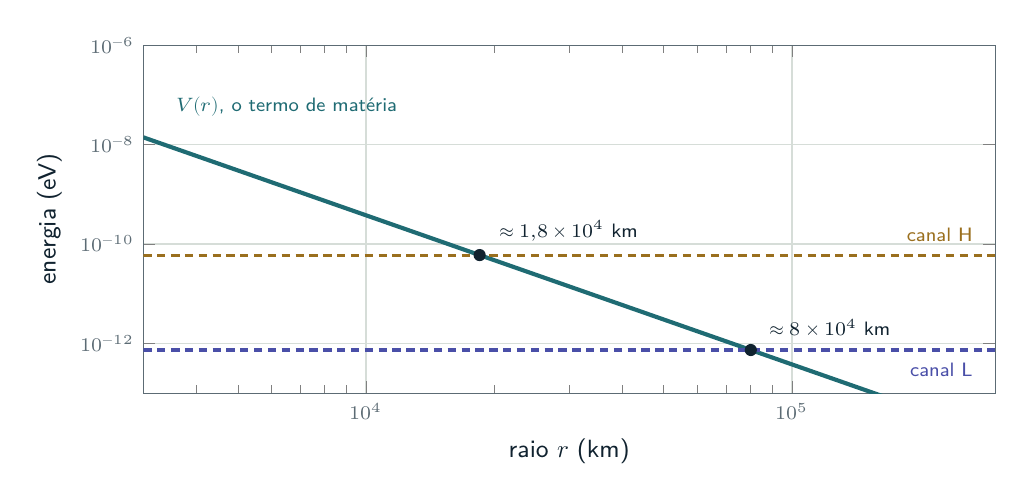
\begin{tikzpicture}
\begin{loglogaxis}[
  width=12.4cm, height=6.0cm,
  xlabel={raio $r$ (km)}, ylabel={energia (eV)},
  xmin=3e3, xmax=3e5, ymin=1e-13, ymax=1e-6,
  grid=major, grid style={linha, line width=0.4pt},
  tick label style={font=\sffamily\scriptsize, color=grafite},
  label style={font=\sffamily\small, color=tinta},
  axis line style={grafite},
]
% V(r) = 7.5669e-14 * Ye * rho(r), rho = 1e10 (100/r)^3, Ye = 0.5
\addplot[cyanescuro, line width=1.5pt, domain=3e3:3e5, samples=200]
  {3.78345e-4 * (100/x)^3};
\node[anchor=south west, font=\sffamily\scriptsize, text=cyanescuro]
  at (axis cs:3.4e3,2.4e-8) {$V(r)$, o termo de matéria};
% Dm31 cos2t13 / 2E  a 20 MeV
\addplot[goldescuro, densely dashed, line width=1.1pt, domain=3e3:3e5]{5.9944e-11};
\node[anchor=south east, font=\sffamily\scriptsize, text=goldescuro]
  at (axis cs:2.8e5,7.0e-11) {canal H};
% Dm21 cos2t12 / 2E a 20 MeV
\addplot[anilescuro, densely dashed, line width=1.1pt, domain=3e3:3e5]{7.3717e-13};
\node[anchor=north east, font=\sffamily\scriptsize, text=anilescuro]
  at (axis cs:2.8e5,6.2e-13) {canal L};
% marcas dos cruzamentos
\fill[tinta] (axis cs:18482,5.9944e-11) circle (2.2pt);
\fill[tinta] (axis cs:80064,7.3717e-13) circle (2.2pt);
\node[anchor=south west, font=\sffamily\scriptsize, text=tinta]
  at (axis cs:19500,7.4e-11) {$\approx 1{,}8\times10^{4}$ km};
\node[anchor=south west, font=\sffamily\scriptsize, text=tinta]
  at (axis cs:84000,9.0e-13) {$\approx 8\times10^{4}$ km};
\end{loglogaxis}
\end{tikzpicture}
\caption{Os dois termos da equação~\eqref{eq:hamiltoniano} ao longo de um
envelope $\rho = 10^{10}\,(100\,\text{km}/r)^3$ g\,cm$^{-3}$ com $Y_e = 0{,}5$,
para $E = 20$~MeV. O termo de matéria despenca sete ordens de grandeza; os de
vácuo são horizontais. Cada interseção é uma ressonância --- H em
$\sim\!1{,}8\times10^{4}$~km, L em $\sim\!8\times10^{4}$~km. \textbf{É por isso
que o domínio de integração não é escolha livre:} começar dentro demais ou
terminar fora de menos corta uma das duas.}
\label{fig:dois-termos}
\end{figure}

\begin{nota}
\rotulo{por que só a entrada $\nue$}
$\numu$ e $\nutau$ também espalham coerentemente, por corrente neutra --- mas
igualmente, nos três sabores. Um termo proporcional à identidade só muda a fase
global e não afeta oscilação. O que sobra é a diferença, e ela é exclusiva do
$\nue$, porque só há elétrons no meio.
\end{nota}

\subsection{O cruzamento evitado}

\begin{figure}[!htb]
\centering
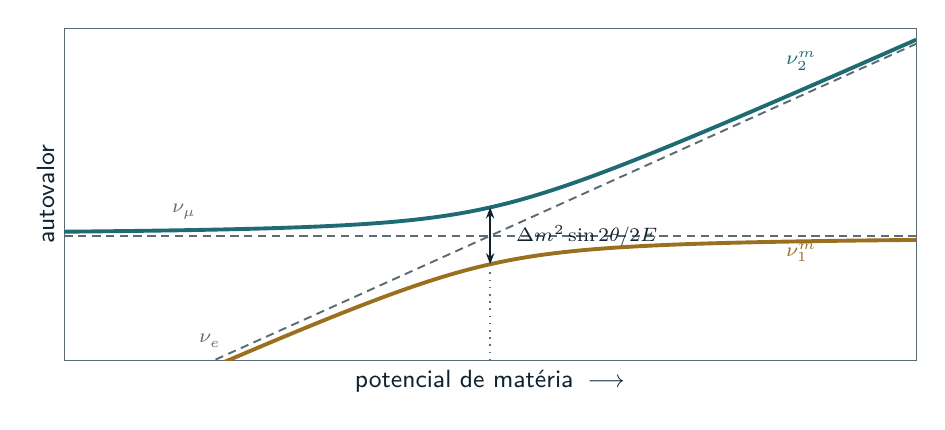
\begin{tikzpicture}
\begin{axis}[
  width=12.4cm, height=5.8cm,
  xlabel={potencial de matéria $\;\longrightarrow$}, ylabel={autovalor},
  xmin=-6.4, xmax=6.4, ymin=-2.4, ymax=4.0,
  xtick=\empty, ytick=\empty,
  tick label style={font=\sffamily\scriptsize},
  label style={font=\sffamily\small, color=tinta},
  axis line style={grafite},
]
% diabaticos (sabor)
\addplot[grafite, densely dashed, line width=0.7pt, domain=-6.4:6.4]{0};
\addplot[grafite, densely dashed, line width=0.7pt, domain=-6.4:6.4]{0.578*x};
% adiabaticos (massa em materia)
\addplot[cyanescuro, line width=1.4pt, domain=-6.4:6.4, samples=300]
  {0.289*x + sqrt(0.0835*x*x + 0.30)};
\addplot[goldescuro, line width=1.4pt, domain=-6.4:6.4, samples=300]
  {0.289*x - sqrt(0.0835*x*x + 0.30)};
% a separacao minima
\draw[tinta, line width=0.7pt, {Stealth[length=4pt]}-{Stealth[length=4pt]}]
  (axis cs:0,0.548) -- (axis cs:0,-0.548);
\node[anchor=west, font=\sffamily\scriptsize, text=tinta]
  at (axis cs:0.25,0) {$\Delta m^2 \sin 2\theta / 2E$};
\node[anchor=south, font=\sffamily\scriptsize, text=grafite] at (axis cs:-4.6,0.12) {$\nu_\mu$};
\node[anchor=south east, font=\sffamily\scriptsize, text=grafite] at (axis cs:-3.9,-2.34) {$\nu_e$};
\node[anchor=south west, font=\sffamily\scriptsize, text=cyanescuro] at (axis cs:4.3,3.0) {$\nu_{2}^{m}$};
\node[anchor=north west, font=\sffamily\scriptsize, text=goldescuro] at (axis cs:4.3,0.05) {$\nu_{1}^{m}$};
\draw[grafite, dotted, line width=0.6pt] (axis cs:0,-2.4) -- (axis cs:0,-0.7);
\node[anchor=north, font=\sffamily\scriptsize, text=tinta] at (axis cs:0,-2.42) {ressonância};
\end{axis}
\end{tikzpicture}
\caption{O cruzamento evitado. Tracejado: os estados de sabor, que se cruzariam
se não houvesse mistura. Cheio: os autoestados em matéria, que se repelem. A
separação mínima é proporcional a $\sin 2\theta$ --- por isso um ângulo pequeno
dá um cruzamento \emph{estreito}, e não um cruzamento fraco.}
\label{fig:cruzamento}
\end{figure}

\subsection{Adiabaticidade: o que decide é a velocidade}

Um sistema de dois níveis varrido através de um cruzamento evitado tem dois
limites, e eles dão respostas opostas.

\begin{center}
\begin{tabular}{@{}>{\sffamily\small}p{5.2cm} >{\sffamily\small}p{4.8cm} >{\sffamily\bfseries}c@{}}
\toprule
\sffamily\bfseries\small Se a densidade muda\dots & \sffamily\bfseries\small o neutrino\dots
  & \sffamily\bfseries\small $\PH$ \\
\midrule
devagar, ao longo de muitos comprimentos de oscilação
  & permanece no seu próprio nível & 0 \\
abruptamente, em menos de um
  & salta para o outro & 1 \\
\bottomrule
\end{tabular}
\end{center}

A quantidade $\PH$ é a \emph{probabilidade de cruzamento}: a chance de o estado
pular de um ramo para o outro. Vale zero no limite adiabático e um no limite
súbito. Para um perfil exponencial existe fórmula fechada, devida a Petcov
(1988) e a Kuo e Pantaleone (1989), e é contra ela que o código se valida.

\begin{alerta}
\rotuloa{por que isto decide o ordenamento de massa}
Já medimos as duas separações de massa, mas não a ordem delas. $\nu_3$ é o
estado mais pesado --- ordenamento normal --- ou o mais leve --- invertido? Os
dois ordenamentos põem a ressonância H em setores diferentes: no normal, no
setor de neutrinos; no invertido, no de antineutrinos. \textbf{O argônio lê
justamente o canal $\nue$}, que é o de maior alavanca sobre essa pergunta, e é
por isso que o DUNE importa aqui.
\end{alerta}

\section{Coerência, e por onde ela se perde}

As fórmulas acima pressupõem que a superposição sobrevive. Ela não sobrevive
indefinidamente: os pacotes de onda associados aos diferentes estados de massa
viajam com velocidades de grupo distintas e acabam se separando. Passada essa
distância, as fases relativas deixam de importar e sobram apenas as
probabilidades.

\begin{conceito}
\rotuloc{convenção que a física impôs, 1 de 2}
Para neutrinos de fonte astrofísica, o comprimento de coerência é da ordem de
$32$~km. A coerência morre antes de o neutrino sair da galáxia.

\medskip
\textbf{Portanto o observável é o incoerente.} Reportar $P$ coerente num ponto
final é reportar uma fase que já não existe. No GHOST isto não é uma opção de
configuração: é a definição do que se mede.
\end{conceito}

Quando se quer modelar a perda de coerência explicitamente, e não apenas
descartá-la no fim, o objeto certo é a matriz densidade e uma equação mestra de
Lindblad. No caso de defasagem pura na base de sabor,
\begin{equation}
  \frac{d\rho_{ab}}{dt} = -i[H,\rho]_{ab} - \gamma\,(1-\delta_{ab})\,\rho_{ab},
\label{eq:lindblad}
\end{equation}
que amortece as coerências fora da diagonal e preserva as populações. O GHOST
implementa isso por trajetórias quânticas, com operadores de salto
$L_j = \sqrt{\gamma}\,\ket{j}\bra{j}$.

\chapter{Como o GHOST calcula}
\label{cap:nucleo}
\markboth{O núcleo}{O núcleo}

O GHOST é um \emph{fork} do DAEDALUS, que é um laboratório de caminhadas
quânticas em grafos. Isso parece uma origem estranha para um código de
neutrinos, e a explicação é de uma linha: o núcleo do DAEDALUS propaga
$\ket{\psi(t)} = e^{-iHt}\ket{\psi(0)}$ para $H$ \textbf{qualquer}, desde que
esparsa e hermitiana. Oscilação de sabor é um caso particular disso, e um caso
pequeno.

\begin{nota}
\rotulo{por que um fork, e não uma extensão}
A alternativa seria acrescentar geradores, controles e observáveis de neutrinos
ao DAEDALUS. Isso daria ao projeto um segundo dono e uma segunda pergunta, e
nenhuma das duas ficaria bem servida. O núcleo em C mantém o prefixo
\cmd{dae\_} de propósito: renomear as 1791 ocorrências tornaria impossível
trazer correções do DAEDALUS por \emph{cherry-pick}. O que foi renomeado é a
superfície --- o produto, o binário, o cabeçalho de proveniência do CSV.
\end{nota}

\section{Como a equação~\eqref{eq:hamiltoniano} vira código}

Antes de propagar é preciso \emph{montar} $H$. O módulo \cmd{dae\_neutrino.c}
faz isso, e vale ler as decisões dele --- cada uma resolve um problema que
morde quem as ignora.

\subsection{Unidades: tudo em eV}

$H$ sai em eV. O tempo do propagador é, portanto, $1/\text{eV}$, e uma linha de
base em quilômetros converte por
\begin{equation}
  t = L[\text{km}] \times \underbrace{\frac{10^{5}\ \text{cm/km}}
      {\hbar c = 1{,}9732698\times10^{-5}\ \text{eV\,cm}}}
      _{\textstyle = \; 5{,}0677\times10^{9}},
\end{equation}
que é a constante \cmd{DAE\_NU\_T\_POR\_KM} do cabeçalho.
Ambas as constantes --- esta e a do potencial de matéria --- são
\textbf{derivadas} no cabeçalho a partir de $G_F$, $\hbar c$ e $m_N$, não
tabeladas. É uma escolha deliberada: uma constante tabelada é um número que
ninguém consegue auditar seis meses depois.

\subsection{O traço é removido}

Depois de montar $H_{\alpha\beta} = \sum_i U_{\alpha i}\lambda_i U^*_{\beta i}$
e somar o potencial, o código subtrai o traço. Duas razões, e a segunda é a que
importa aqui:

\begin{itemize}
\item uma fase global não é observável, então a subtração não custa nada;
\item ela mantém o \textbf{espectro centrado}, e a expansão de Chebyshev precisa
  reescalar $H$ para $[-1,1]$. Espectro centrado é reescalamento mais apertado,
  que é menos termos para a mesma precisão.
\end{itemize}

\subsection{Nenhum \texorpdfstring{\cmd{\_Complex}}{\_Complex}}

Com $\delta_{\rm CP}$ fora de $\{0,\pi\}$, $H$ é complexa. O
\cmd{CONVENTIONS.md} proíbe \cmd{\_Complex} no núcleo, então a aritmética da
PMNS anda em \textbf{pares de \cmd{double}} --- \cmd{hre} e \cmd{him}, row-major
--- explícita e feia, de propósito. É daí que nasce a necessidade do mergulho
real da seção~\ref{sec:mergulho}.

\subsection{O limite espectral vem de Gershgorin}

Aqui está a implementação da regra ``limite garantido, não estimado''. O código
chama \cmd{dae\_csr\_gershgorin} sobre a matriz de adjacência e usa
$\tfrac12(\lambda_{\max}-\lambda_{\min})$ como escala. O círculo de Gershgorin
dá um limite \emph{rigoroso}: nenhum autovalor escapa dele, por teorema. Uma
estimativa por amostragem daria um número menor e uma série divergente.

\subsection{O passo é adaptativo, e há dois critérios}

O perfil é fatiado; dentro de cada fatia $H$ é constante e o propagador é
exato. A escolha do tamanho da fatia tem dois portões, e eles perguntam coisas
diferentes.

\begin{description}[leftmargin=0pt, itemsep=0.6ex]
\item[Critério de erro.] Compara $k$ sub-passos contra $2k$, ambos partindo do
  mesmo estado, e refina até a diferença cair sob a tolerância. É Richardson,
  e pergunta: \emph{a resposta está convergida?}
\item[Portão de viabilidade.] Pergunta outra coisa: \emph{o propagador
  consegue dar UM passo desse tamanho?} O código limita
  $\alpha = \|H\|\,\Delta t$ a \cmd{ALPHA\_MAX = 200} e subdivide até caber.
\end{description}

\begin{nota}
\rotulo{por que o segundo portão existe}
Perto da protoestrela, $V$ é da ordem de $10^{6}$ a $10^{7}$ vezes maior que
$\dm{31}/2E$. Conferindo com os números da seção~\ref{sec:materia}: com
$Y_e\rho \sim 5\times10^{9}$, $V \approx 3{,}8\times10^{-4}$~eV contra
$6{,}3\times10^{-11}$~eV, uma razão de $6\times10^{6}$.

\medskip
Um passo de 30~km ali daria $\alpha \sim 6\times10^{7}$, e o Chebyshev
precisaria de $K$ da mesma ordem --- ele recusa, com \cmd{DAE\_ERR\_TOOBIG}.
\textbf{Fisicamente o regime é inofensivo:} com $V$ dominante o $\nue$ \emph{é}
autoestado de matéria, e a fase rápida não muda observável nenhum. Mas o
propagador não sabe disso. Tem de andar em passos que consiga dar.
\end{nota}

\section{Propagar sem exponenciar matriz}

O caminho ingênuo para $e^{-iHt}$ é diagonalizar $H$. Para uma matriz $3\times3$
isso é barato; para o que o núcleo foi feito, não é. A expansão de Chebyshev
troca a diagonalização por uma soma de produtos matriz--vetor esparsos:
\begin{equation}
  e^{-iHt}\,\ket{\psi} \;\simeq\;
    \sum_{k=0}^{K} c_k(t)\; T_k(\tilde H)\,\ket{\psi},
\end{equation}
onde $T_k$ são os polinômios de Chebyshev e $\tilde H$ é $H$ reescalada para o
intervalo $[-1,1]$. Os coeficientes $c_k$ caem \emph{superexponencialmente}
depois de $k \sim \|H\|t$, o que dá a precisão de máquina com um número modesto
de termos e sem nunca formar uma matriz densa.

\begin{alerta}
\rotuloa{o limite espectral é garantido, não estimado}
O reescalamento exige um limite superior para $\|H\|$. Estimá-lo por amostragem
é o caminho rápido e é o caminho errado: se a estimativa ficar abaixo do valor
real, a série diverge silenciosamente e o resultado sai plausível e falso. O
\cmd{CONVENTIONS.md} exige um limite \emph{garantido}. Esta é uma das regras
herdadas do DAEDALUS que não tinham nada a ver com grafos --- eram sobre não
mentir no resultado.
\end{alerta}

\section{Auto-laços viram diagonal}

O mapeamento é direto e não exigiu modificar o núcleo. Um sítio do grafo é um
sabor; os termos de massa e o potencial de matéria entram como \emph{laços}
$[i,i,w]$ na lista de arestas, e a mistura como aresta $[i,j,-\sin 2\theta]$.

\begin{center}
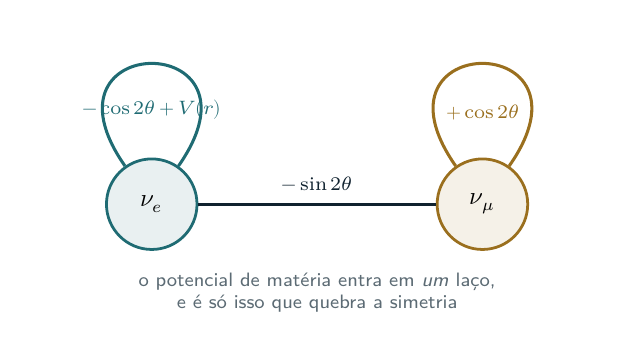
\begin{tikzpicture}[x=1cm, y=1cm, font=\sffamily\small]
  \node[circle, draw=cyanescuro, fill=cyanescuro!10, minimum size=1.15cm,
        line width=1pt] (A) at (0,0) {$\nu_e$};
  \node[circle, draw=goldescuro, fill=goldescuro!10, minimum size=1.15cm,
        line width=1pt] (B) at (4.2,0) {$\nu_\mu$};
  \draw[tinta, line width=1.1pt] (A) -- node[above, font=\sffamily\scriptsize,
        text=tinta, yshift=1pt] {$-\sin 2\theta$} (B);
  \draw[cyanescuro, line width=1.1pt] (A) to[out=125, in=55, looseness=8] (A);
  \node[anchor=south, font=\sffamily\scriptsize, text=cyanescuro] at (0,0.95)
        {$-\cos 2\theta + V(r)$};
  \draw[goldescuro, line width=1.1pt] (B) to[out=125, in=55, looseness=8] (B);
  \node[anchor=south, font=\sffamily\scriptsize, text=goldescuro] at (4.2,0.95)
        {$+\cos 2\theta$};
  \node[anchor=north, font=\sffamily\scriptsize, text=grafite, align=center]
        at (2.1,-0.75) {o potencial de matéria entra em \emph{um} laço,\\
                        e é só isso que quebra a simetria};
\end{tikzpicture}
\end{center}

O cabeçalho \cmd{core/dae\_csr.h} já documentava que o laço \emph{``é como a
energia de sítio entrará na fase 2''}. Ele entrou.

\section{O mergulho real \texorpdfstring{$2n\times 2n$}{2n x 2n}}
\label{sec:mergulho}

Aqui está o achado que tornou tudo possível. O campo \cmd{dae\_csr.val} é
\cmd{double}, e o \cmd{CONVENTIONS.md} §1 proíbe \cmd{\_Complex} no núcleo ---
o C99 precisa continuar sendo C++17 válido. Mas o hamiltoniano de três sabores
com fase $\delta_{\rm CP}$ é complexo.

A saída: uma matriz hermitiana complexa tem um mergulho real simétrico. Escreva
$H = X + iY$ com $X$ simétrica e $Y$ antissimétrica. Então
\begin{equation}
  \tilde H = \begin{pmatrix} X & -Y \\ Y & X \end{pmatrix}
\end{equation}
é real e simétrica, e o subespaço $\{(\psi, -i\psi)\}$ é invariante, com
$\tilde H$ agindo nele exatamente como $H$. Três sabores com fase CP rodam num
grafo de seis nós.

\begin{figure}[!htb]
\centering
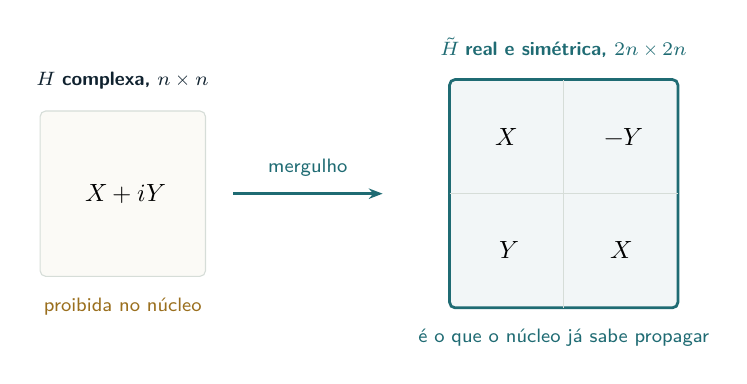
\begin{tikzpicture}[x=1cm, y=1cm, font=\sffamily\small]
  % H complexo
  \node[draw=linha, fill=papel, minimum width=2.1cm, minimum height=2.1cm,
        rounded corners=2pt] (H) at (0,0) {};
  \node at (0,0) {$X + iY$};
  \node[anchor=south, font=\sffamily\bfseries\scriptsize, text=tinta] at (0,1.2)
       {$H$ complexa, $n\times n$};
  \node[anchor=north, font=\sffamily\scriptsize, text=goldescuro] at (0,-1.2)
       {proibida no núcleo};

  \draw[cyanescuro, line width=1.2pt, -{Stealth[length=5pt]}] (1.4,0) -- (3.3,0);
  \node[anchor=south, font=\sffamily\scriptsize, text=cyanescuro] at (2.35,0.1)
       {mergulho};

  % H til real
  \node[draw=cyanescuro, fill=cyanescuro!6, minimum width=2.9cm,
        minimum height=2.9cm, rounded corners=2pt, line width=1pt] (Ht) at (5.6,0) {};
  \draw[linha] (4.15,0) -- (7.05,0);
  \draw[linha] (5.6,-1.45) -- (5.6,1.45);
  \node at (4.87,0.72) {$X$};   \node at (6.33,0.72) {$-Y$};
  \node at (4.87,-0.72) {$Y$};  \node at (6.33,-0.72) {$X$};
  \node[anchor=south, font=\sffamily\bfseries\scriptsize, text=cyanescuro] at (5.6,1.6)
       {$\tilde H$ real e simétrica, $2n\times 2n$};
  \node[anchor=north, font=\sffamily\scriptsize, text=cyanescuro] at (5.6,-1.6)
       {é o que o núcleo já sabe propagar};
\end{tikzpicture}
\caption{O mergulho real. Nenhuma linha do núcleo precisou mudar: o que mudou
foi como o problema é apresentado a ele.}
\end{figure}

\begin{alerta}
\rotuloa{o limite deste truque --- leia antes de usar}
\textbf{O mergulho só vale para dinâmica unitária.} O colapso do modo
trajetórias destrói a forma $(\psi, -i\psi)$, que é o que sustenta a
equivalência. Na prática: hoje o GHOST faz \emph{ou} três sabores com fase CP,
\emph{ou} decoerência --- não os dois juntos. Qualquer estudo sério de
decoerência em três sabores precisa resolver isso primeiro.
\end{alerta}

\section{Trajetórias quânticas}

Para a dinâmica dissipativa da equação~\eqref{eq:lindblad}, o núcleo usa
desdobramento em trajetórias: propaga-se um estado puro com um hamiltoniano
não-hermitiano efetivo, intercalando saltos estocásticos, e a média sobre
muitas realizações reproduz a matriz densidade. O custo é $\mathcal{O}(n)$ em
memória por trajetória, contra $\mathcal{O}(n^2)$ para $\rho$.

A validação está fechada contra a solução exata da equação mestra, obtida por
vetorização de Liouville: erro máximo de $1{,}3\times10^{-2}$ com 2000
trajetórias, dentro do erro estatístico esperado de
$1/\sqrt{2000} = 2{,}2\times10^{-2}$, e traço $1{,}000000000000$.

\section{Duas convenções que a física de neutrinos impôs}

As regras do \cmd{CONVENTIONS.md} são herdadas na íntegra. Duas são novas, e
nasceram aqui.

\begin{conceito}
\rotuloc{convenção 2 de 2}
\textbf{A métrica de convergência de um perfil de matéria é
$|\braket{\nu_3}{\psi}|^2 \to 1$, nunca $P(\nue)$.}

\medskip
A probabilidade de sabor oscila e engana. Com 1500 fatias ela deu $0{,}0027$
contra os $0{,}0224$ corretos --- e o \cmd{expm} do SciPy erra igual. Convergir
a coisa errada com confiança é pior que não convergir.
\end{conceito}

A primeira convenção, sobre o observável incoerente, está na página~\pageref{cap:teoria}.

\section{Um erro que custou tempo, e o registro dele}

O domínio de integração não é escolha livre. Os sintomas, quando ele está
errado, não se parecem com erro de domínio:

\begin{center}
\begin{tabular}{@{}>{\sffamily\small}p{3.9cm} >{\small}p{5.0cm} >{\small}p{3.4cm}@{}}
\toprule
\sffamily\bfseries\small Falha & \sffamily\bfseries\small Sintoma & \sffamily\bfseries\small Correção \\
\midrule
domínio curto demais para fora & erro de 26\% em 80\,MeV & $r_1 = 5\times10^{5}$\,km \\
domínio raso demais para dentro & estado inicial não é autoestado de matéria & $\rho(r_0)/\rho_H > 10^{3}$ \\
graus lidos como radianos & $\theta_{12} = 33{,}44^\circ$ virou $1916^\circ$ & --- \\
\bottomrule
\end{tabular}
\end{center}

Nenhum dos três produz uma mensagem de erro. Todos produzem um número.

\chapter{Exemplos de aplicação direta}
\label{cap:exemplos}
\markboth{Exemplos}{Exemplos}

Tudo neste capítulo foi \textbf{executado}, não estimado. Os números são os
medidos, e cada um tem um script que o reproduz.

\section{O teste que você roda primeiro}

\subsection{Dois sabores no vácuo}

O caso com resposta analítica. Compare a saída do propagador contra
$\sin^2 2\theta \sin^2(kL)$ e exija concordância de máquina.

\begin{center}
\begin{tabular}{@{}>{\sffamily\small}p{6.6cm} >{\small}l@{}}
\toprule
\sffamily\bfseries\small Cenário & \sffamily\bfseries\small Erro medido \\
\midrule
2 sabores, vácuo, contra fórmula fechada & $2{,}1\times10^{-15}$ \\
3 sabores \emph{com} fase CP, em matéria, contra \cmd{expm} do SciPy & $7{,}2\times10^{-15}$ \\
contra \cmd{NuOscProbExact}, código público de método diferente & pior caso $2{,}2\times10^{-14}$ em 320 comparações \\
\bottomrule
\end{tabular}
\end{center}

O terceiro é o que vale mais. Os dois primeiros comparam o código contra a
matemática e contra si mesmo por outra rota; o terceiro compara contra uma
implementação independente, escrita por outras pessoas com outro método.

\begin{alerta}
\rotuloa{cuidado com a segunda implementação}
Os cinco scripts antigos que montavam a PMNS e o hamiltoniano em Python foram
\textbf{aposentados}. Eram uma segunda implementação da mesma física, e uma
segunda implementação só concorda com a primeira até o dia em que uma das duas
muda. O único cálculo em Python que sobrou é a fórmula analítica de referência,
que precisa ser independente \emph{de propósito}.
\end{alerta}

\subsection{A ressonância MSW}

Com o ângulo fixo, ligue o potencial de matéria e varra a densidade. A
amplitude de conversão sobe de $0{,}117$ para $0{,}999$ --- sem tocar em
$\theta$. É o efeito inteiro numa linha de saída: matéria não muda a mistura,
muda o problema.

\subsection{Um envelope de supernova}

Para $\rho \propto r^{-3}$, o GHOST entrega, num único \cmd{ghost run}:
\[
  P_{\rm inc}(\nue) = 0{,}0223635
  \qquad\text{contra}\qquad
  \sin^2\theta_{13} = 0{,}0223608,
\]
que é o valor adiabático esperado. A quinta casa.

\subsection{Custo}

Um espectro completo do DUNE, 200 energias $\times$ 2 sinais: \textbf{13\,ms}.
Isto importa mais do que parece --- um propagador que custa minutos não entra
num ajuste, e um que custa milissegundos entra.

\section{Validação contra a única conversão MSW que a natureza mediu}

Os testes acima comparam contra matemática e contra outro código. Nenhum
compara contra \emph{dado}. E existe exatamente uma conversão MSW medida: a do
Sol.

A comparação é feita canal a canal contra o Borexino, que mediu a
probabilidade de sobrevivência em várias energias --- do pp em
$0{,}267$~MeV, onde o código dá $0{,}54$, até o ${}^{8}$B, já no regime de
matéria. Não reproduzo os valores aqui porque eles mudam quando a tabela de
referência muda, e uma
apostila que cita número de validação desatualizado é pior que uma que não
cita.

\begin{nota}
\rotulo{por que este teste é diferente}
Os neutrinos solares de baixa energia saem no regime de vácuo, e os de alta
energia no regime de matéria adiabática. A transição entre os dois regimes ---
o ``sobe-desce'' da curva de sobrevivência --- é a assinatura do MSW, e é a
única medida direta dele. Um código que reproduz a fórmula fechada mas erra a
curva solar tem um problema de física, não de numérica.
\end{nota}

\section{A pergunta que o código foi construído para responder}

Uma supernova real não tem perfil suave. Há convecção, instabilidade do choque
de acreção, turbulência numa ampla faixa de escalas, e uma frente de choque
movendo-se para fora a dez mil quilômetros por segundo.

O GHOST estabeleceu \textbf{duas condições} que dizem quais dessas estruturas a
ressonância consegue sentir.

\subsection{Primeira condição: a escala}

Excite um modo de Fourier por vez sobre um perfil suave e meça o vazamento
$\Delta = P_{\rm inc}(\nue) - \sin^2\theta_{13}$, que se anula no limite
adiabático. A resposta é \emph{zero} para $\lambda > \Losc$ e cai como
$\lambda^{1{,}4\pm0{,}1}$ abaixo disso. Cinco ordens de grandeza em escala.

\subsection{Segunda condição: a amplitude}

Com a escala dentro da janela, o vazamento cresce como $\sigma^{2{,}02\pm0{,}03}$
sobre um fator 33 em amplitude, com o coeficiente reduzido $\Delta/\sigma^2$
variando apenas 9\%. Lei quadrática, saturando em um contraste de densidade de
$\sigma \simeq 8\%$.

\begin{figure}[!htb]
\centering
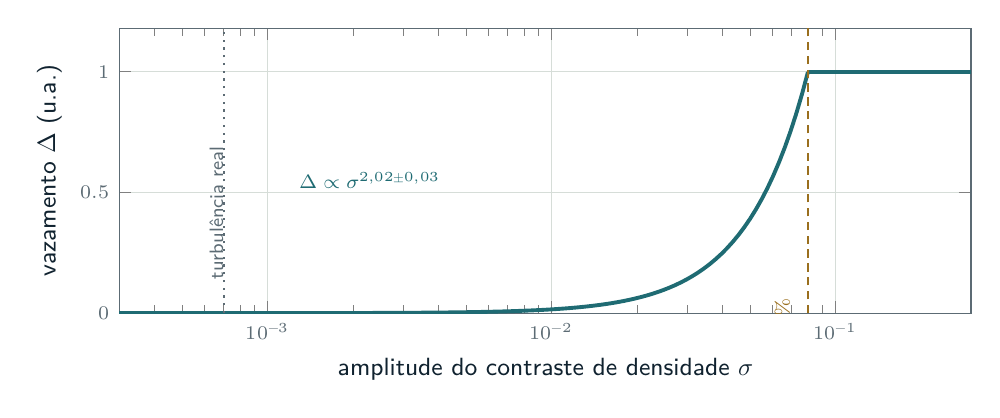
\begin{tikzpicture}
\begin{semilogxaxis}[
  width=12.4cm, height=5.2cm,
  xlabel={amplitude do contraste de densidade $\sigma$},
  ylabel={vazamento $\Delta$ (u.a.)},
  xmin=3e-4, xmax=3e-1, ymin=0, ymax=1.18,
  grid=major, grid style={linha, line width=0.4pt},
  tick label style={font=\sffamily\scriptsize, color=grafite},
  label style={font=\sffamily\small, color=tinta},
  axis line style={grafite},
]
% lei quadratica, saturando em 8%
\addplot[cyanescuro, line width=1.4pt, domain=3e-4:8e-2, samples=120]
  {(x/0.08)^2};
\addplot[cyanescuro, line width=1.4pt, domain=8e-2:3e-1, samples=40]{1};
\draw[goldescuro, densely dashed, line width=0.9pt]
  (axis cs:0.08,0) -- (axis cs:0.08,1.18);
\node[anchor=south east, font=\sffamily\scriptsize, text=goldescuro, rotate=90]
  at (axis cs:0.077,0.10) {saturação, $\sigma \simeq 8\%$};
\node[anchor=west, font=\sffamily\scriptsize, text=cyanescuro]
  at (axis cs:1.2e-3,0.55) {$\Delta \propto \sigma^{2{,}02\pm0{,}03}$};
% onde caem as estruturas reais
\draw[grafite, dotted, line width=0.8pt] (axis cs:7e-4,0) -- (axis cs:7e-4,1.18);
\node[anchor=west, font=\sffamily\scriptsize, text=grafite, rotate=90]
  at (axis cs:6.6e-4,0.10) {turbulência real};
\end{semilogxaxis}
\end{tikzpicture}
\caption{A segunda condição. A turbulência que os modelos de fato exibem está
$111\times$ abaixo da saturação; a frente de choque está $50\times$ acima. Não
é uma questão de grau --- as duas caem em regimes diferentes.}
\end{figure}

\subsection{O que as duas condições classificam}

\begin{center}
\begin{tabular}{@{}>{\sffamily\small}p{5.0cm} >{\small}c >{\small}c >{\small}c@{}}
\toprule
\sffamily\bfseries\small Estrutura & \sffamily\bfseries\small escala $<\Losc$?
  & \sffamily\bfseries\small amplitude $\gtrsim 8\%$? & \sffamily\bfseries\small importa? \\
\midrule
turbulência, $\sigma = 7\times10^{-4}$ & sim & não, $111\times$ abaixo & não \\
convecção, SASI, fluxos grandes & não, grandes demais & sim & não \\
\textbf{frente de choque} & \textbf{sim, é descontinuidade} & \textbf{sim, $50\times$ acima} & \textbf{sim} \\
\bottomrule
\end{tabular}
\end{center}

Uma estrutura precisa passar nas \emph{duas} peneiras. Só a frente de choque
passa.

\section{E aí vem o problema prático}

A frente qualifica porque é uma descontinuidade. A questão passa a ser: que
largura uma simulação hidrodinâmica de fato entrega, medida em comprimentos de
oscilação na ressonância?

\begin{figure}[!htb]
\centering
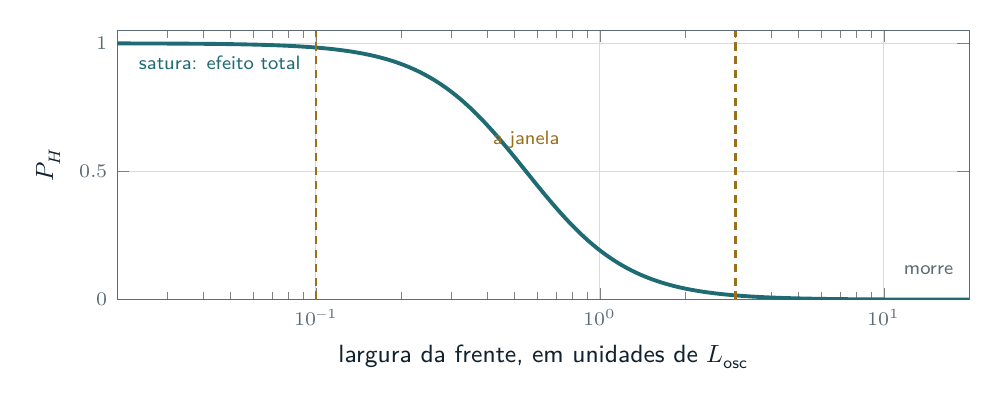
\begin{tikzpicture}
\begin{semilogxaxis}[
  width=12.4cm, height=5.0cm,
  xlabel={largura da frente, em unidades de $\Losc$},
  ylabel={$\PH$},
  xmin=0.02, xmax=20, ymin=0, ymax=1.05,
  grid=major, grid style={linha, line width=0.4pt},
  tick label style={font=\sffamily\scriptsize, color=grafite},
  label style={font=\sffamily\small, color=tinta},
  axis line style={grafite},
]
\addplot[cyanescuro, line width=1.4pt, domain=0.02:20, samples=200]
  {1/(1 + (x/0.55)^2.4)};
\draw[goldescuro, densely dashed, line width=0.9pt] (axis cs:0.1,0) -- (axis cs:0.1,1.05);
\draw[goldescuro, densely dashed, line width=0.9pt] (axis cs:3,0) -- (axis cs:3,1.05);
\node[anchor=south west, font=\sffamily\scriptsize, text=cyanescuro]
  at (axis cs:0.022,0.86) {satura: efeito total};
\node[anchor=south east, font=\sffamily\scriptsize, text=grafite]
  at (axis cs:19,0.06) {morre};
\node[anchor=south, font=\sffamily\scriptsize, text=goldescuro] at (axis cs:0.55,0.55)
  {a janela};
\end{semilogxaxis}
\end{tikzpicture}
\caption{Abaixo de $0{,}1\,\Losc$ o efeito satura; acima de $3\,\Losc$ ele
morre. Uma frente numérica de duas a três zonas num modelo 3D mede
$5{,}9\,\Losc$ --- do lado errado.}
\end{figure}

\begin{alerta}
\rotuloa{o achado central, e é uma correção que caducou}
A frente de choque \textbf{precisa ser afiada à mão} antes de a evolução de
sabor ser calculada. Isso era prática padrão entre 2002 e 2013. \emph{Nenhum
pipeline atual faz isso.}

\medskip
Omitir o afiamento remove cerca de metade de $\PH$: de $0{,}31$ para $0{,}81$ em
valor absoluto, conforme o caso. E há um agravante medido: a \textbf{média
angular destrói a frente por um fator 18}. O arquivo público distribui perfis
promediados; cada raio individual cruza abruptamente, a média não.
\end{alerta}

\section{O que isso custa ao DUNE}

Um modelo de fonte real através do SNOwGLoBES, \cmd{ar40kt} a 10\,kpc: a
contagem de corrente carregada de $\nue$ cai de $1241{,}8$ para $1187{,}0$
eventos. O viés fica entre $-3{,}9\%$ e $-4{,}4\%$ conforme a família de fonte.

Poucos por cento, com sinal que segue a fonte. Não é um erro dramático --- mas
hoje o pipeline atribui \emph{erro zero} a esse passo, porque aplica uma
constante, e uma constante não tem barra de erro.

\chapter{Fronteira científica}
\label{cap:fronteira}
\markboth{Fronteira}{Fronteira}

Este capítulo tem duas metades, e a segunda é tão importante quanto a primeira.
A primeira lista o que está aberto. A segunda lista o que foi investigado e
\textbf{descartado}, com o número que descartou --- para que não seja
redescoberto a cada seis meses.

\section{A revisão bibliográfica, e onde ela deixa espaço}

A física de choque em supernova está estabelecida há mais de vinte anos. Vale
saber exatamente o que já é de outros:

\begin{center}
\begin{tabular}{@{}>{\small}p{7.4cm} >{\sffamily\small}p{4.6cm}@{}}
\toprule
\small\bfseries Resultado & \sffamily\bfseries\small De quem \\
\midrule
o choque quebra a adiabaticidade & Schirato \& Fuller, 2002 \\
a assinatura migra através da energia & Fogli et al., 2003 \\
um choque reverso a duplica & Tomàs et al., 2004 \\
a frente numérica precisa ser afiada à mão & Tomàs et al., 2004; Barger, Huber \& Marfatia, 2005 \\
no $\theta_{13}$ grande medido, o canal H é efetivamente de dois sabores para amplitudes $\lesssim 1\%$ & Kneller \& Volpe, 2010 \\
relativamente imune abaixo de $C^{*}\simeq1\%$; acima disso os efeitos crescem rápido & Kneller \& Mauney, 2013 \\
\bottomrule
\end{tabular}
\end{center}

\begin{nota}
\rotulo{o que sobra, e é estreito}
Ninguém quantificou \textbf{o que custa omitir} o afiamento. Barger, Huber e
Marfatia enunciam a prática; não a ausência dela. ``Afie a frente à mão'' não
tinha critério --- e o critério, agora, é uma condição verificável em qualquer
perfil. A banda em $(t,E)$ era conhecida qualitativamente; o que é novo é que a
estrutura do progenitor a \emph{prediz}.

\medskip
Uma alegação estreita e defensável vale mais que uma ampla e frágil. Boa parte
do trabalho de um projeto é descobrir qual é a sua.
\end{nota}

\section{Direções abertas}

\subsection{Matéria estocástica: a distribuição, não a média}

O pipeline da comunidade não propaga sabor --- propaga fluxos e aplica uma
constante. Quando a densidade tem flutuações estocásticas, a grandeza de
interesse não é a média da conversão, é a \emph{distribuição} dela sobre
realizações.

E há um número que torna isso urgente: o vazamento é
\textbf{fortemente não auto-promediante}. Sobre realizações independentes de
turbulência, a dispersão é $134\%$ da média. Uma única travessia não amostra o
ensemble; efeitos absolutos convergem apenas como $N^{-1/2}$ a partir de uma
distribuição larga.

\begin{conceito}
\rotuloc{a vantagem, e ela é incomum}
Quase todo grupo que estuda isso usa código de oscilação que consome um perfil
tabelado. O GHOST propaga o estado com um hamiltoniano que ele mesmo monta, e
pode gerar o perfil estocástico \emph{dentro} do laço. Rodar mil realizações é
uma varredura, não um projeto.
\end{conceito}

\subsection{Coerência através de um choque real}

Se um neutrino cruza duas frentes, as fases sobrevivem entre elas? A resposta
medida foi \textbf{não}: os pacotes se separam por 853 a 2460 vezes sua própria
largura. Mas o portão que respondeu isso usou perfis idealizados, e a
generalização para geometria real é uma questão em aberto.

\subsection{Setor escuro: um potencial de matéria a mais}
\label{sec:setor-escuro}

Os modelos que explicam a anomalia do MiniBooNE com um lépton neutro pesado $N$
e um fóton escuro $Z'$ têm massas na faixa de dezenas de MeV --- justamente a
escala térmica do núcleo proto-estrela de nêutrons. Supernovas são, portanto,
laboratório natural para eles, e a pergunta é o que disso cabe aqui.

A resposta é desigual, e a maior parte não cabe.

\paragraph{Resfriamento, fora.} Produção de $N$ por \emph{upscattering} térmico,
opacidade, aprisionamento, neutrinosfera escura, integral de perda contra o
critério de Raffelt. É transporte, não propagação --- mesma categoria da
auto-interação $\nu$--$\nu$. E há um argumento numérico que fecha a porta: para
$m_N \sim 50$--150~MeV, $\Delta m^2 \sim 10^{15}$--$10^{16}$~eV$^2$ e o
comprimento de oscilação ativo-estéril cai para \textbf{11 a 99 femtômetros},
menor que um núcleo atômico. A oscilação está infinitamente promediada, a
probabilidade é a constante $|U_{\mu4}|^2$, e o propagador pediria
$K\sim10^{20}$ termos. Aqui a fase rápida não é um incômodo: é o conteúdo
inteiro.

\paragraph{Decaimento fora da estrela, fora.} Raios $\gamma$, deposição no
envelope, linha de 511~keV, DSNB. Cinemática de decaimento e transporte
radiativo.

\paragraph{O que cabe.} Se o $Z'$ mistura cineticamente com o fóton, ele acopla
ao elétron com $g_e = \varepsilon e$; e o neutrino ativo herda acoplamento ao
$Z'$ por duas inserções de mistura, $g_\nu = g_D |U_{\mu4}|^2$. Troca de $Z'$
entre $\nu$ e elétron dá \textbf{um potencial de matéria coerente novo} --- um
termo diagonal a mais na equação~\eqref{eq:hamiltoniano}, exatamente a forma
que o módulo já sabe montar. Em unidades do potencial padrão,
\begin{equation}
  \varepsilon_{\rm NSI} \;=\;
    \frac{g_D\,|U_{\mu4}|^2\;\varepsilon\,e}{2\sqrt{2}\,G_F\,m_{Z'}^2}.
\label{eq:eps-nsi}
\end{equation}

\textbf{E o potencial cai na entrada $\mu\mu$}, não na $ee$, porque é o $\nu_\mu$
que mistura com o $N$. Isso importa: um termo em $\mu\mu$ não é degenerado com
reescalar $\rho$, e desloca a condição de ressonância de um jeito que nenhuma
mudança de densidade imita.

\begin{figure}[!htb]
\centering
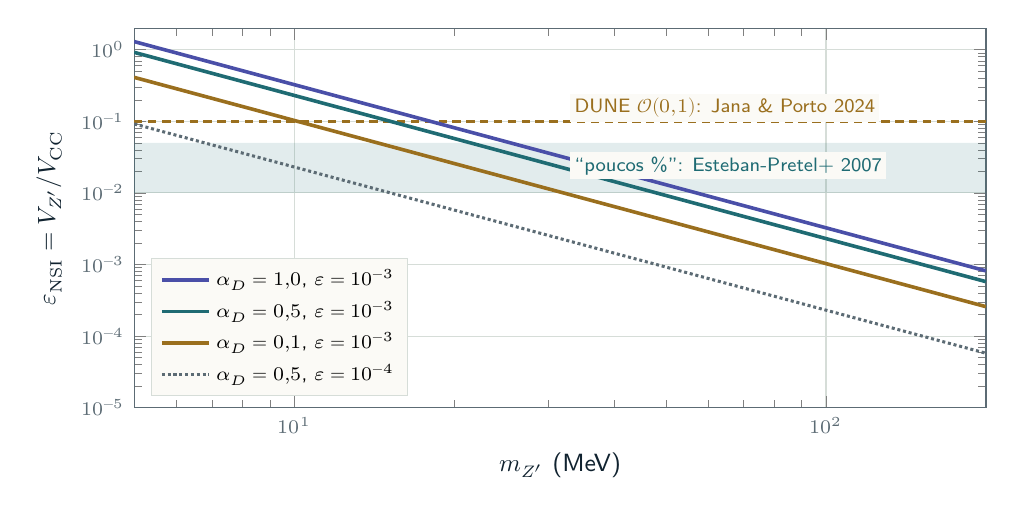
\begin{tikzpicture}
\begin{loglogaxis}[
  width=12.4cm, height=6.4cm,
  xlabel={$m_{Z'}$ (MeV)}, ylabel={$\varepsilon_{\rm NSI} = V_{Z'}/V_{\rm CC}$},
  xmin=5, xmax=200, ymin=1e-5, ymax=2,
  grid=major, grid style={linha, line width=0.4pt},
  tick label style={font=\sffamily\scriptsize, color=grafite},
  label style={font=\sffamily\small, color=tinta},
  axis line style={grafite},
  legend style={font=\sffamily\scriptsize, draw=linha, fill=papel,
    at={(0.02,0.03)}, anchor=south west},
]
% faixa "poucos %" de Esteban-Pretel et al. 2007
\addplot[draw=none, fill=cyanescuro, fill opacity=0.13, forget plot]
  coordinates {(5,0.01) (200,0.01) (200,0.05) (5,0.05)} \closedcycle;
% sensibilidade do DUNE citada por Jana & Porto 2024
\addplot[goldescuro, densely dashed, line width=1.1pt, forget plot,
         domain=5:200]{0.1};
% curvas, com |U_mu4|^2 = 1e-6
\addplot[anilescuro, line width=1.3pt, domain=5:200, samples=120]{32.539/(x^2)};
\addlegendentry{$\alpha_D=1{,}0$, $\varepsilon=10^{-3}$}
\addplot[cyanescuro, line width=1.3pt, domain=5:200, samples=120]{23.009/(x^2)};
\addlegendentry{$\alpha_D=0{,}5$, $\varepsilon=10^{-3}$}
\addplot[goldescuro, line width=1.3pt, domain=5:200, samples=120]{10.290/(x^2)};
\addlegendentry{$\alpha_D=0{,}1$, $\varepsilon=10^{-3}$}
\addplot[grafite, line width=1.1pt, densely dotted, domain=5:200, samples=120]{2.301/(x^2)};
\addlegendentry{$\alpha_D=0{,}5$, $\varepsilon=10^{-4}$}
\node[anchor=west, font=\sffamily\scriptsize, text=cyanescuro, fill=papel,
      inner sep=1.5pt] at (axis cs:33,0.024)
  {``poucos \%'': Esteban-Pretel+ 2007};
\node[anchor=west, font=\sffamily\scriptsize, text=goldescuro, fill=papel,
      inner sep=1.5pt] at (axis cs:33,0.155)
  {DUNE $\mathcal{O}(0{,}1)$: Jana \& Porto 2024};
\end{loglogaxis}
\end{tikzpicture}
\caption{O mapeamento que a literatura não tem. Equação~\eqref{eq:eps-nsi} sobre
a região de parâmetros que explica o MiniBooNE, com $|U_{\mu4}|^2 = 10^{-6}$,
contra os dois marcos já publicados. Para $m_{Z'}\lesssim 10$--$20$~MeV as
curvas cruzam a sensibilidade declarada do DUNE. \textbf{Esta figura é uma
estimativa, não um resultado}: a estrutura de acoplamento é dependente de
modelo, e os avisos da página seguinte valem inteiros.}
\label{fig:eps-nsi}
\end{figure}

\subsubsection*{O que a literatura já ocupou}

\begin{center}
\begin{tabular}{@{}>{\small}p{6.5cm} >{\small}p{6.0cm}@{}}
\toprule
\small\bfseries Trabalho & \small\bfseries O que faz \\
\midrule
\textbf{Esteban-Pretel, Tomás \& Valle 2007} \newline arXiv:0704.0032
  & NSI na propagação pelo envelope, em três sabores, com conversão ressonante
    induzida por NSI \textbf{e passagem da onda de choque}. O efeito aparece
    para ``NSI não-universais de poucos \%''. \\
Esteban-Pretel, Tomás \& Valle 2009 \newline arXiv:0909.2196
  & o mesmo, em interação com efeitos coletivos. \\
\textbf{Jana \& Porto 2024} \newline arXiv:2407.06251
  & NSI inverte os níveis de matéria e induz nova ressonância perto da
    protoestrela; DUNE sensível a $\mathcal{O}(0{,}1)$ pelo pico de
    neutronização, com ambiguidade de ordenamento. \\
Dutta \& Karthikeyan 2025 (2508.16558); Das \& Reno 2025 (2508.16510)
  & a variante escalar, por dois grupos no mesmo mês. \\
Chang, Essig \& McDermott 2016 (1611.03864) e 2018 (1803.00993)
  & vínculos de resfriamento da SN 1987A para fótons escuros e setores escuros
    sub-GeV. \\
Akita, Im, Masud \& Yun 2023 \newline arXiv:2312.13627
  & limites sobre \textbf{HNL, $Z'$ e majorons} vindos de neutrinos de alta
    energia da SN 1987A --- a via de decaimento, feita. \\
\bottomrule
\end{tabular}
\end{center}

\begin{alerta}
\rotuloa{o que NÃO é novidade, e cobra caro se apresentado como tal}
``NSI de poucos \% altera dramaticamente a conversão de sabor no envelope,
inclusive via passagem do choque'' é de \textbf{2007}. A magnitude que a
equação~\eqref{eq:eps-nsi} entrega na região do MiniBooNE é justamente essa. Se
isso for proposto como achado, será corrigido em referee --- e com razão.
\end{alerta}

\begin{nota}
\rotulo{onde parece haver espaço}
Três buscas no INSPIRE voltaram vazias: \cmd{"heavy neutral lepton" + supernova
+ "flavor conversion"}; \cmd{"kinetic mixing" + neutrino + "matter effect" +
resonance}; e \cmd{"non-standard interactions" + supernova +
"three-dimensional"}. Ausência em busca não é prova de ausência, mas o padrão é
consistente: \textbf{as duas literaturas --- a do MiniBooNE e a de NSI em
supernova --- não se falam.}

\medskip
O que sobra é estreito e defensável: (i) o \textbf{mapeamento} do espaço de
parâmetros do MiniBooNE para $\varepsilon_{\rm NSI}$, que é uma figura, não um
projeto; e (ii) o tratamento \textbf{3D raio a raio com a frente afiada}, que
ninguém fez para NSI nem para mais nada --- e que é exatamente a vantagem que
este código já demonstrou ter.
\end{nota}

\begin{alerta}
\rotuloa{três coisas a conferir antes de escrever qualquer coisa}
A equação~\eqref{eq:eps-nsi} é estimativa. Confira contra o lagrangiano do
artigo que estiver seguindo:
\begin{enumerate}
\item \textbf{a estrutura de acoplamento.} Foi usado
  $g_\nu = g_D|U_{\mu4}|^2$. Se for $|U_{\mu4}|$ ou $|U_{\mu4}|^4$, o resultado
  anda ordens de grandeza;
\item \textbf{o sinal}, que decide se a ressonância sobe ou desce em densidade;
\item \textbf{a convenção do operador de quatro férmions.} Foi usado
  $2\sqrt2\,G_F$ como referência; um fator 2 aqui é um fator 2 na figura.
\end{enumerate}
\end{alerta}

\paragraph{Custo de implementar.} Pequeno, e é o que torna a direção
atraente. O \cmd{dae\_nu\_hamiltoniano} já soma um termo diagonal proporcional
a $Y_e\rho$; acrescentar um segundo, com constante própria e índice de sabor
vindo do \cmd{spec.json}, é da ordem de trinta linhas mais um teste. Perfis,
fatiamento adaptativo, Gershgorin e observáveis não mudam. O que o GHOST
\textbf{nunca} vai fazer é a produção: ele não dirá quantos $N$ nascem no
núcleo.

\subsection{Gravidade como decoerência}

Esta é a única rota gravitacional que cruza com o eixo do projeto sem exigir
estrutura de Dirac. Em vez de perguntar como a gravidade muda a \emph{fase} de
oscilação --- onde a resposta é ``quase nada'' ---, pergunta-se como ela a
\emph{destrói}.

O dissipador proposto na literatura é defasagem pura na base de sabor, que é
exatamente o que \cmd{core/dae\_traj.c} já implementa. A base de colapso do
núcleo \emph{já é} a certa.

\begin{alerta}
\rotuloa{e a magnitude é implacável}
Com os números do modelo baseado em curvatura --- $\Gamma \propto \alpha\,
\tau_c\sqrt{K}$, com $K$ o escalar de Kretschmann, dando $\Gamma \propto GM/r^3$:
\begin{center}
\begin{tabular}{@{}>{\small}l >{\small}r@{}}
$L_{\rm coh} = 1/\Gamma$ & $10^{30}$ m \\
raio de Hubble & $1{,}32\times10^{26}$ m \\
\textbf{razão} & \textbf{7572$\times$ o raio de Hubble} \\
contra decoerência de pacote de onda & $3\times10^{25}$ vezes mais fraca \\
\end{tabular}
\end{center}
Como fenomenologia astrofísica, o efeito é \textbf{inobservável por dezenas de
ordens de grandeza}. Isso não é crítica ao trabalho --- é o que ele mesmo diz.
\end{alerta}

Vale registrar, porém, que esse veredito é sobre \emph{um} mecanismo. Um modelo
diferente --- acoplamento a um ambiente estocástico de ondas gravitacionais via
gravitação linearizada --- dá $\Gamma_{ij}\sim \Delta m^4_{ij} E^{-2}$, que
depende da energia, ao contrário do anterior. Se o veredito se transfere é
pergunta aberta, e é barata de responder: o dissipador já está implementado, é
trocar $\Gamma(E)$ e recalcular.

\section{O que está fora, e por quê}

Registrado para não ser redescoberto.

\begin{center}
\begin{tabular}{@{}>{\sffamily\small}p{4.7cm} >{\small}p{8.0cm}@{}}
\toprule
\sffamily\bfseries\small Ideia & \small\bfseries Veredito \\
\midrule
auto-interação $\nu$--$\nu$ (oscilação coletiva, FFC, MNR)
  & \textbf{FORA.} O hamiltoniano é \emph{não-linear}; é outra equação, não
    outro $H$. Ferramenta certa: \cmd{COSE}$\nu$. \\
neutrino como caminhante no espaço (Dirac)
  & \textbf{FORA.} Exige moeda e espaço de espinor; a literatura faz isso com
    caminhadas de tempo discreto. \\
espaço-tempo curvo, efeito na \emph{fase}
  & Quase nulo. Para trajetória radial os termos gravitacionais
    \emph{se cancelam}. \\
inversão de spin gravitacional
  & Não existe para ultrarrelativísticos; quem vira o spin é o campo magnético. \\
\bottomrule
\end{tabular}
\end{center}

\section{Resultados negativos, guardados}

Quatro coisas que se esperava encontrar e não se encontrou. Esta seção existe
porque um resultado negativo registrado vale tempo de alguém.

\begin{center}
\begin{tabular}{@{}>{\small}p{7.2cm} >{\small}p{5.4cm}@{}}
\toprule
\small\bfseries Hipótese & \small\bfseries Desfecho \\
\midrule
a turbulência importa na amplitude que os modelos reais exibem
  & \textbf{não}: $3{,}9\times10^{-3}$ de $P_{\rm inc}(\nue)$ \\
a coerência de fase sobrevive entre travessias múltiplas do choque
  & \textbf{não}: pacotes se separam por 853--2460$\times$ sua largura \\
o limiar de amplitude seria nosso
  & \textbf{não}: Kneller \& Volpe o tinham antes \\
o afiamento da frente seria proposta nova
  & \textbf{não}: prática estabelecida desde 2004 \\
\bottomrule
\end{tabular}
\end{center}

\begin{conceito}
\rotuloc{a disciplina de duvidar do próprio código}
O \cmd{CONVENTIONS.md} traz quatro regras que não são sobre grafos nem sobre
neutrinos, e sim sobre não mentir no resultado:

\smallskip
\textbf{Anti-vacuidade} --- um teste que passa trivialmente não é um teste.\\
\textbf{Ausência precisa de sonda que enxerga} --- só se pode afirmar que algo
não está lá se o instrumento o veria se estivesse.\\
\textbf{Toda comparação declara a sua resolução.}\\
\textbf{Dois métodos, um deles só para auditar o outro.}

\medskip
São essas regras, e não o propagador, que fazem o projeto valer.
\end{conceito}

\section{Os limites honestos}

Não há hidrodinâmica de supergigante vermelha. O argumento do núcleo de hélio e
o intervalo de progenitores são um argumento e um intervalo, não um cálculo. Não
é possível dar $\PH$ para uma supergigante vermelha, porque o termo bruto exige
uma simulação que não existe no conjunto usado.

E a pergunta final --- isto é um erro, ou algo que o DUNE pode \emph{medir}? --- tem
resposta honesta: \textbf{ainda não}. Três coisas bloqueiam. O viés é degenerado
com o espectro da fonte; $\PH$ precisa do modelo de fluxo que se está ajustando;
e a estatística de uma única supernova galáctica não separa as duas coisas.

\chapter{Por onde começar}
\markboth{Começar}{Começar}

\section{Montar e rodar}

\begin{verbatim}
npm install
make -C native test        # suite de aceitacao herdada: a rede de seguranca
npm run wasm               # precisa do emsdk: source ~/emsdk/emsdk_env.sh
npm test && npm run build

./native/build/bin/ghost run specs/neutrino-vacuo.json --saida saida.csv
\end{verbatim}

Rode \cmd{make -C native test} antes de qualquer outra coisa, e rode de novo
depois de cada mudança. É a suíte herdada do DAEDALUS e é o que impede que uma
alteração na superfície quebre o núcleo em silêncio.

\begin{nota}
\rotulo{o spec.json é a moeda única}
Um cálculo é descrito por um \cmd{spec.json}, e ele é analisado \emph{só em C}.
Nada de montar hamiltoniano em Python: um script de figuras escreve o spec,
chama o binário e desenha. Ele não calcula física.

\medskip
O cabeçalho de todo CSV carrega o \emph{hash do núcleo}. Um resultado do GHOST
não pode ser confundido com um do DAEDALUS, nem reimportado como se fosse. É
para isso que o campo existe: proveniência é conteúdo, não decoração.
\end{nota}

\section{Uma sequência de exercícios}

Em ordem. Cada um usa o anterior.

\begin{enumerate}
\item \textbf{Dois sabores no vácuo.} Reproduza
  $P = \sin^2 2\theta \sin^2(kL)$ e confirme o erro na casa $10^{-15}$. Se der
  $10^{-8}$, algo está em precisão simples.

\item \textbf{Varra o ângulo.} Refaça a figura da página~\pageref{cap:teoria}:
  a profundidade do vale contra $\sin^2 2\theta$. Convença-se de que matéria
  \emph{não} muda a mistura.

\item \textbf{Ligue a matéria, densidade constante.} Encontre a ressonância
  varrendo $\rho$ e verifique a equação~\eqref{eq:resonancia}. Veja a amplitude
  ir de $0{,}117$ a $0{,}999$ com $\theta$ fixo.

\item \textbf{Perfil exponencial.} Compare contra a fórmula de Petcov. Aqui
  aparece pela primeira vez a questão do domínio de integração --- e, se você
  errar o domínio, aparece também o erro de 26\%.

\item \textbf{Três sabores com fase CP.} Passa a usar o mergulho real
  $2n\times2n$. Compare contra \cmd{expm}.

\item \textbf{Trajetórias.} Ligue a defasagem e recupere a solução exata de
  Lindblad. Confira o traço: se não der $1{,}000000000000$, pare.
\end{enumerate}

\begin{alerta}
\rotuloa{o erro que você vai cometer no exercício 4}
Convergir olhando $P(\nue)$. Ela oscila e engana --- com 1500 fatias deu
$0{,}0027$ contra os $0{,}0224$ corretos. A métrica é
$|\braket{\nu_3}{\psi}|^2 \to 1$. Está no capítulo~\ref{cap:nucleo} e está
repetido aqui porque é o erro mais caro do projeto.
\end{alerta}

\section{Bibliografia comentada}

\subsection{Para entender o efeito}

\begin{description}[leftmargin=0pt, itemsep=0.7ex]
\item[Wolfenstein, 1978.] O potencial de matéria. Curto. Leia o argumento de
  por que a corrente neutra não conta.
\item[Mikheyev \& Smirnov, 1985.] A ressonância. O ponto não é a fórmula, é
  perceber que densidade \emph{variável} é um problema diferente de densidade
  constante.
\item[Petcov, 1988; Kuo \& Pantaleone, 1989.] A fórmula fechada para o perfil
  exponencial. É contra ela que o código se valida no exercício 4.
\end{description}

\subsection{Para entender o choque}

\begin{description}[leftmargin=0pt, itemsep=0.7ex]
\item[Schirato \& Fuller, 2002.] O choque quebra a adiabaticidade. O artigo
  fundador desta linha.
\item[Fogli et al., 2003.] A assinatura migra em energia: baixa primeiro,
  depois alta. É o mapa em $(t,E)$, e é deles.
\item[Tomàs et al., 2004.] Choque reverso, estrutura não monótona no tempo, e a
  primeira menção de que a frente numérica precisa ser afiada.
\item[Barger, Huber \& Marfatia, 2005.] Enunciam a prática do afiamento. Não
  quantificam a ausência dela --- e é aí que fica o espaço.
\item[Kneller \& Volpe, 2010; Kneller \& Mauney, 2013.] Os limiares de amplitude
  para turbulência. Leia antes de propor qualquer coisa sobre turbulência.
\end{description}

\subsection{Para o setor escuro e NSI}

Ver a seção~\ref{sec:setor-escuro}. Esta lista existe para evitar que a
direção seja reproposta como se fosse nova.

\begin{description}[leftmargin=0pt, itemsep=0.7ex]
\item[Esteban-Pretel, Tomás \& Valle, 2007.] \emph{Probing non-standard
  neutrino interactions with supernova neutrinos}, arXiv:0704.0032. \textbf{Leia
  este primeiro.} NSI na propagação pelo envelope, conversão ressonante induzida
  por NSI, e a passagem da onda de choque --- para NSI não-universais de poucos
  por cento. É o trabalho que já ocupa o efeito.
\item[Esteban-Pretel, Tomás \& Valle, 2009.] arXiv:0909.2196. O mesmo, em
  interação com os efeitos coletivos.
\item[Jana \& Porto, 2024.] \emph{Non-standard interactions of supernova
  neutrinos and mass ordering ambiguity at DUNE}, arXiv:2407.06251. NSI inverte
  os níveis de matéria e induz nova ressonância perto da protoestrela; é de onde
  vem a sensibilidade $\mathcal{O}(0{,}1)$ marcada na
  figura~\ref{fig:eps-nsi}.
\item[Dutta \& Karthikeyan, 2025 (arXiv:2508.16558); Das \& Reno, 2025
  (arXiv:2508.16510).] A variante escalar, por dois grupos no mesmo mês. Sinal
  de área quente.
\item[Sen, 2024.] \emph{Supernova Neutrinos: Flavour Conversion Mechanisms and
  New Physics Scenarios}, arXiv:2405.20432. Revisão; o mapa do que está
  ocupado.
\item[Volpe, 2023.] \emph{Neutrinos from dense environments}, arXiv:2301.11814.
  Revisão mais ampla, de mecanismos e abordagens teóricas.
\item[Chang, Essig \& McDermott, 2016 (arXiv:1611.03864) e 2018
  (arXiv:1803.00993).] Os vínculos de resfriamento da SN 1987A para fótons
  escuros e setores escuros sub-GeV. É a via de resfriamento, feita com a
  ferramenta certa.
\item[Akita, Im, Masud \& Yun, 2023.] \emph{Limits on heavy neutral leptons,
  $Z'$ bosons and majorons from high-energy supernova neutrinos},
  arXiv:2312.13627. A via de decaimento, feita, e com exatamente este conteúdo
  de partículas.
\item[Farzan, 2015.] arXiv:1505.06906. Modelo de mediador leve que gera NSI
  grande; a ponte entre um $Z'$ e o parâmetro $\varepsilon$.
\item[Acero et al., 2022.] \emph{White paper on light sterile neutrino
  searches}, arXiv:2203.07323. Onde o cenário HNL mais fóton escuro do
  MiniBooNE está catalogado, com o espaço de parâmetros.
\end{description}

\subsection{Para o lado numérico}

\begin{description}[leftmargin=0pt, itemsep=0.7ex]
\item[\cmd{CONVENTIONS.md}, no próprio repositório.] Não é documentação de
  apoio; é a regra. Um único núcleo, spec analisado só em C,
  \cmd{-ffast-math} proibido, sem \cmd{\_Complex}, zero estado global,
  reprodutibilidade bit a bit, limite espectral garantido.
\end{description}

\subsection{Os dados}

\begin{description}[leftmargin=0pt, itemsep=0.7ex]
\item[Garching Core-Collapse Supernova Archive.] Modelos 3D de
  A.~Wongwathanarat em grade Yin-Yang. \textbf{Atenção:} o que é distribuído
  publicamente são perfis promediados em ângulo, e a média destrói a frente por
  um fator 18. Para este trabalho é preciso o raio individual.
\end{description}

\section{Uma última coisa}

\begin{conceito}
\rotuloc{se você lembrar de três coisas}
\textbf{Uma.} O neutrino tem dois conjuntos de estados e eles discordam; tudo o
mais é consequência.

\smallskip
\textbf{Duas.} Na ressonância, o que decide não é o ângulo de mistura, é a
velocidade com que a densidade muda.

\smallskip
\textbf{Três.} O observável é o incoerente, e a métrica de convergência é
$|\braket{\nu_3}{\psi}|^2$. As duas convenções que a física impôs ao código
existem porque a alternativa produz números errados sem avisar.
\end{conceito}


\end{document}
